\newpage
\topskip0pt
\vspace*{\fill}
\section*{Abstract}
Disturbance has been suggested as an important promotor of species coexistence, and the intermediate disturbance hypothesis (IDH) suggests that diversity should be maximised at intermediate levels of disturbance. However, the mechanism by which disturbance is increased is often not explicitly stated in studies, or is a composite measure containing many different aspects of disturbance. We use a stochastic lottery-type model to demonstrate that among species competing for light along a fecundity-juvenile growth trade-off, a) disturbance can increase or decrease diversity;  b) the aspect of disturbance (intensity or frequency) that is measured can make a dramatic difference to the qualitative results obtained; and these results are robust to changes in system capacity (the number of individuals the system is capable of maintaining), and also productivity.
\vspace*{\fill}
% \PACS{PACS code1 \and PACS code2 \and more}
% \subclass{MSC code1 \and MSC code2 \and more}
\newpage
\section{Introduction}
\label{intro}
One of the most persistent issues in ecology is how some communities, such as tropical forests, grasslands and coral reefs maintain high levels of species diversity. Some mechanisms such as resource partitioning \citep[e.g.][]{sala1989resource,schoener1974resource} and the storage effect \citep{warner1985coexistence} are widely recognised, while several previous studies \citep[e.g.][]{denslow1987tropical,sousa1984role} have suggested that disturbance events may play an important part in promoting diversity in some systems. Disturbance, that is, events that result in the death of large number of individuals and alter niche opportunities \citep{shea2004moving}, creates an environment that prevents the exclusion of weaker competing species, such as pioneer species. If levels of disturbance are too low, these pioneer-like species will be excluded, whereas if disturbance levels are too high they will drive strong competitors with slow recruitment, for example late successional tree species, to extinction. Thus only at intermediate disturbance levels is it possible for both early- and late- successional species to coexist. It is on these arguments that the intermediate disturbance hypothesis (IDH) suggests that intermediate levels of disturbance allow the maximal level of species diversity \citep[e.g.][]{connell1978diversity,huston1979general}, producing a peaked diversity-disturbance relationship (DDR).

The IDH was proposed to address the specific issue of tree diversity in tropical forests and fish and coral diversity in coral reefs \citep{connell1978diversity}, but can also be traced back to \cite{grime1973competitive}. Despite this long history, because disturbances often occur infrequently, and because in many communities individuals may be relatively long-lived it has been hard to test the IDH and empirical studies have shown mixed results \citep[see review in ][]{mackey2001diversity}. Some support for the IDH has been found \citep[e.g.][]{biswas2010disturbance,molino2001tree,rogers1993hurricanes} while other studies reject the hypothesis \citep[e.g.][]{hubbell1999light,huxham2000field}. \cite{bongers2009intermediate} find that diversity does indeed peak at intermediate disturbance levels, but they also conclude that disturbance does not contribute much to diversity, especially in wet or moist forests.

It has been argued that there are at least three different axes upon which disturbances should be measured: frequency; area affected; and intensity \citep{malanson1984intensity,miller1982community,sousa1984role}.  However, many empirical studies consider disturbance levels in forests as a single parameter, such as the total area lost in a given time period (effectively frequency multiplied by intensity) \citep[e.g.][]{molino2001tree,nakagawa2000impact,peterson1997tornado}. Fire ecology studies have often acknowledged the difference between different factors influencing fire, such as ignition probability and spread \citep[e.g.][]{kilgore1979fire,turner1994landscape}, observing that most fires are of low intensity and high frequency \citep{kilgore1979fire}, while spatial connectedness has an impact on overall fire intensity \citep{turner1994landscape}. \cite{svensson2009equal} found that equal levels of total disturbance can have different effects. However, there remain relatively few theoretical studies that consider the relative impact of frequency and intensity of disturbances \citep[but see ][]{miller2011frequency}. In an early review of the empirical literature, \cite{denslow1980patterns} \textbf{indicated} that communities that have infrequent but large patches cleared through disturbance \textbf{can} be more diverse than those that suffer frequent, but small-scale disturbances (e.g. gaps created by tree-fall). \cite{hartshorn1978treefalls} reported that in a Costa Rican forest most disturbances are caused by relatively small gaps appearing after a tree falls and that as a consequence the forest is dominated by shade-tolerant species. In a recent theoretical study, \cite{miller2011frequency} show how disturbance intensity and frequency have different effects on community dynamics and the emergence of the IDH depends greatly on the combination of the two. It seems likely that this may be a significant factor behind the relative lack of consensus on whether or not the classical IDH pattern is general in nature communities.

Productivity of a system is also known to have a significant effect on disturbance; \cite{kondoh2001unifying} used the dynamic equilibrium model of \cite{huston1979general} to demonstrate theoretically that an increase in productivity leads to an increase the disturbance levels that give peak diversity.

Here we build on this work and consider the effects of disturbance frequency and intensity separately in a two species forest model, in which there is a fecundity-growth trade-off \textbf{with system capacity as a parameter}. Analyses of the model confirm that the frequency and intensity of the disturbance can have significantly different effects, and that the emergence of the IDH is dependent upon the combination of disturbance intensity and frequency. We also demonstrate that thee results are robust to changes in system capacity and productivity.

\section{The Model}
\label{model}
We consider a simple lottery type model, originally introduced by \cite{sale1978coexistence} and \cite{chesson1981environmental} and used extensively since \citep[e.g.][]{muko2000species,pacala1992herbivores}. There are a fixed number $N$ distinct sites, each capable of supporting a single adult individual, observed in continuous time $\tau$. At discrete times $\tau_1,\tau_2, \dots$, there is a tree death, selected at random from the community, followed by competition between the remaining individuals for the vacated site. We assume that the time to fill a gap with an individual is small enough that the gap created at time $\tau_t$ is filled by an adult individual by time $\tau_{t+1}$, i.e. death-replacement events are sufficiently far apart temporally that they do not overlap and can be considered as discrete events. This assumption makes it possible to model this system as a time homogeneous Markov Chain (MC) model. With the range of parameters considered below, the expected gap replenishment time is approximately 4 years. Simulations reducing the number of adult trees by 4\% (consistent with 1\% annual mortality for this replenishment period) do not exhibit any qualitative difference.

Gaps are occupied by populations of two species $N_1(t), N_2(t)$, such that $N_1(t) + N_2(t) = N$, where $t$ represents time as measured by the number of replacement events that have occurred, i.e. $N_i(t)$ represents the population of species $i$ after the gap created at time $\tau_t$ has been filled, and before another gap is created at time $\tau_{t+1}$. Because after each death-replacement event, the number of individuals is fixed, we consider the dynamics of species 1 only, modelling $N_1(t)=n$ with $N_2(t)=N-n$. We assume 
\begin{enumerate}
\item The system is closed, so no seeds are introduced from elsewhere. Biologically, this could suggest an island population or community isolated by other geographic constraints. A low level of immigrating seeds does not qualitatively affect the results.
\item The individuals considered are asexual or self-fertilising, so that a single individual can produce seeds, and that individuals are always reproductively active.
\item The two species differ only in growth rates $g_i$ and annual per capita seed production $s_i$, with a trade-off between competitive ability (growth) and colonisation ability (seed numbers). Species 2 has the higher growth rate of the two species, $g_2>g_1$, while species 1 is the more fecund $s_1>s_2$. Note that if this trade-off is relaxed, such that $s_2\geq s_1$, coexistence is impossible, with species 2 dominating. We note that species 2 is in effect seed limited as it would win more sites if it were able to send seeds there; whereas species 1 is competitor limited and would gain proportionally more sites if species 2 were rare.
\item As individuals compete for light in a gap, we assume complete asymmetric competition. Once the combined size of the juveniles in a gap is that of a single adult, then the largest individual will win the site. Competition for a site is therefore a race to reach size $C/2$, where $C$ is the size of an adult individual.
\item It is possible for the faster growing species 2 to usurp juveniles of the slower growing species. The initial juvenile to reach a gap is determined by lottery, but species 2 may take over the site if further seeds arrive before a species 1 juvenile has grown sufficiently large. To usurp species 1, species 2 requires seeds to arrive before species 1 has been present for time $x=C(1/g_2-1/g_1)/2$.
\item Seeds are all assumed to be viable and are dispersed at random in the environment by a homogeneous Poisson process (with rate $\lambda_i =s_iN_i(t)/N$) as per high distance dispersals in \cite{clark1999interpreting}.
\item Disturbance events occur at each time step with probability $f=(dNT_D)^{-1}$ where $T_D$ is the expected number of years between disturbance events, and $d$ is the expected annual mortality rate (fixed at $1\%$). Within these events, individuals are killed with probability $I$ (the intensity of the disturbance), before the remaining individuals compete to fill the emptied sites. Increasing either frequency $f$ or intensity $I$ will result in an increase in total basal area lost over a given time frame, a standard measure of disturbance \citep[e.g.][]{molino2001tree,peterson1997tornado}.
\end{enumerate}
When a disturbance does not occur (with probability $1-f$), the number of species 1 individuals will increase if a species 2 individual dies, seeds from species 1 reach the site first, and then grow for time $x$ without species 2 reaching the site. As both species have the same dispersal kernel, this gives
\begin{align}
\label{increase}
P(\text{Increase}(n))&=P(N_1(1)=n+1)|N_1(0)=n) \\
&=\frac{N-n}{N}\frac{s_1 n}{s_1 n +s_2(N-n-1)}\exp \left( -s_2 \frac{N-n-1}{N} x\right),\notag \end{align}
where the exponential term is the probability that no species 2 seeds arrive in time $x$. Similarly, species 1 will decline in numbers if it suffers a death, and species 2 claims the site, either arriving at the site first or by successfully invading a site where species 1 juveniles are present, giving
\begin{align}
\label{decrease}
P(\text{Decrease}(n))=&P(N_1(1)=n-1 | N_1(0)=n)  \\ 
=&\frac{n}{N}\frac{s_2 (N-n)}{s_1 (n-1) +s_2(N-n)} \notag \\
& + \frac{n}{N}\frac{s_1 (n-1)}{s_1 (n-1) +s_2(N-n)}\left(1-\exp \left( -s_2 \frac{N-n}{N} x\right)\right). \notag \end{align}
All other possibilities result in the populations of the two species remaining the same after a time step, so we use a third function $P(\text{Stay}(n))=1-P(\text{Increase}(n))-P(\text{Decrease}(n))$ to fully define the transition probabilities, giving a $(N+1) \times (N+1)$ tridiagonal transition matrix $A$, with $A_{i,i}=P(\text{Stay}(i-1)), A_{i,i+1}=P(\text{Increase}(i-1)), A_{i,i-1}=P(\text{Decrease}(i-1))$.

During a disturbance event, each individual has a probability $I$ of mortality, resulting in $d_{dist}=d_1+d_2$ total deaths, where $d_i$ is the number of species $i$ deaths. The remaining $N-d_{dist}$ individuals compete over the empty site, with species 1 colonising if it reaches the site at least time $x$ before species 2. Therefore, species 1 will take a site with a probability defined by the function
\begin{equation}
\label{sp1}
Sp_1(n_1^*,n_2^*)=\frac{s_1 n_1^*}{s_1n_1^*+s_2n_2^*}\exp \left(-s_2 x\frac{n_2^*}{N}\right),
\end{equation}
where $n_1^*,n_2^*$ are the populations remaining immediately after the deaths from a disturbance event.

We will also relax \textbf{assumption 2 listed above;} that each individual is reproductively active all the time, which has the effect of reducing the productivity of the system. Instead, each time a gap is contested, we suppose that each individual is producing seeds with probability $p$. \textbf{This parameter $p$ is assumed to be time invariant and independent of species abundance, as well as constant across species.} This allows us to consider the effects of seed limitation, which we compare with other ways of altering productivity.

DOES THIS BIT FLOW FROM PARA TO PARA RIGHT?

A standard tool for measuring coexistence in a stochastic model is to find an everywhere positive and steady probability distribution. Such a steady distribution is ecologically relevant only if it is stable. However, in the case where the model has absorbing boundaries, and the probability of reaching those boundaries is greater than zero, the only steady state distributions are those absorbing boundaries, where a species exists in monoculture. 

Since the model is stochastic, and the boundaries are absorbing, the long-term expectation is for a monoculture where one or other species goes extinct. Of course, it may take a long time to reach these boundaries. We therefore consider a variant of invasion analysis, similar to that introduced by \cite{chesson1989invasibility} and \cite{ellner1989convergence}. \cite{chesson1982stabilizing} proved that when the boundary growth rates, or average changes at the boundaries are positive, such that each species will on average increase when rare, the populations are stochastically bounded away from zero, and coexistence is expected. Note that because the model presented here uses a discrete state space, the invasion criteria are considered with a single individual of the invader present, as opposed to being assessed at 0 as in a continuous state space. We approximate the expected change at the boundaries ($n=1,N-1$) using the formula
\begin{equation}
\label{avchange}
\begin{array}{rl}
\text{AverageChange}(n) = (1-f)\left[P(\text{Increase}(n))-P(\text{Decrease}(n))\right]&\\[0.75em]
+ f\left[ NI Sp_1(n(1-I)) - nI\right]&.
\end{array}
\end{equation}
\textbf{The first term in \eqref{avchange} is the expected change when disturbance does not occur multiplied by the within-event probability that there is no disturbance event. The second term indicates the expected change during a disturbance as measured by the expected remaining populations. Due to Jensen's inequality, this is not the actual expected change, but an approximation.} This approximation improves as system capacity $N$ is increased, as demonstrated in Appendix~\ref{app2a}, and works well for $N\geq500$. \textbf{Coexistence is predicted for regions of parameter space} where the following 2 inequalities both hold;
\begin{align}
\label{ac1}\text{AverageChange}(1)&>0, \\
\label{acn-1}\text{AverageChange}(N-1)&<0. \end{align}
Note that when there is no disturbance ($T_D=\infty$), these conditions simplify to 
\begin{align}
\label{lowerboundarycond}P(\text{Increase}(1))&>P(\text{Decrease}(1)) \\
\label{upperboundarycond}P(\text{Increase}(N-1))&<P(\text{Decrease}(N-1)). \end{align}
In biological terms, these conditions can be considered as the following: If there is a single individual of a species remaining, for that species to persist it must produce offspring that successfully colonise at least one other site before the adult dies. We implicitly assume that either individuals are asexual, or that self-fertilisation is possible, and more complex models are required to investigate sexual populations that are self-incompatible. The colonisation of a second site therefore must be more likely than the death of this single individual. Analyses using these conditions are extensively checked against time series simulations.

\section{Results} \label{results}
\subsection{Coexistence without disturbances ($T_D=\infty$)}
\label{ss:resultshomo}

Substituting in the probabilities that populations increase or decrease from \eqref{increase} and \eqref{decrease} into the conditions given by \eqref{lowerboundarycond} and \eqref{upperboundarycond}, coexistence of both species occurs when the growth rate factor $x$ falls in the range
\begin{equation}
\label{xrange}
x_{min}=\frac{N\ln\left(\frac{s_1(N-1)}{s_1(N-2)+s_2}\right)}{s_2}<x<\frac{N\ln\left(\frac{s_1(N-1)}{s_1+s_2(N-2)}\right)}{s_2(N-2)}=x_{max}.
\end{equation}
Note $x_{min}$ and $x_{max}$ are both positive, since $s_1>s_2$ and $g_1<g_2$.  Extensive numerical simulations of the MC confirm this to be a good approximation of the range of coexistence.

If the growth rates satisfy \eqref{xrange} then the model state tends to move away from the boundary, which results in  the survival of both species around a quasi-equilibrium where the probabilities of increasing and decreasing species 1 numbers are identical. \textbf{A quasi-equilibrium as discussed here is defined to be the point $n^*$ at which the expected change is towards that value from both below and above, i.e.}
\begin{equation}
\text{AverageChange}(n)\begin{cases}
<0 & n>n^*, \\
>0 & n<n^*. \end{cases} \end{equation}
 When $x$ falls below $x_{min}$, the growth advantage of species 2 is not sufficient to overcome the disadvantage it has when colonising sites, and it experiences extinction while species 1 persists in monoculture. When $x$ is above $x_{max}$, then the growth disadvantage of species 1 is too severe for it to survive, and species 2 eventually claims all sites. Within this range, however, long-term survival of both species is likely, and those time series simulations that do display extinction will often show a long transient prior to a stochastically driven extinction event. \textbf{Figure~\ref{fig:ttevx} shows the increase in expected time to extinction within this range of parameters.}

The range of growth rates that give coexistence given by \eqref{xrange} is dependent on system capacity $N$. For small $N$, an initial increase in system capacity widens the range of $x$ for which coexistence is possible. The likelihood of both species surviving for given parameter values $s_1,s_2,x$ increases for two reasons. First, there is now a greater region of parameter space that will support the long term survival of both species. Second, there is also a longer transient prior to extinction, as the average distance of a population from the boundary increases simply by virtue of there being more possible states. 
 However, as $N$ increases, the range given by \eqref{xrange} asymptotes to a fixed range that  depends on the fecundity of the two species given by
\begin{equation}
\label{bignxrange}
\frac{1}{s_2}-\frac{1}{s_1}<x<\frac{\ln\left(\frac{s_1}{s_2}\right)}{s_2}.
\end{equation}  
The variation of $x_{min}$ and $x_{max}$ with system capacity $N$ is shown in Figure~\ref{fig:systemsize}. \textbf{For all $s_1/s_2<30$, the values of $x_{min},x_{max}$ are very closely approximated by \eqref{bignxrange} whenever $N\geq 500$}. We therefore conclude that system capacity has limited effect on the population dynamics \textbf{of most undisturbed forests. Effects such as founder control, where species cannot coexist and the identity of the surviving species is determined by the initial populations, can only occur in small or fragmented environments.}
 However, Appendix~\ref{app2b} shows the time taken to reach equilibrium increases with system capacity, \textbf{and this has some limited consequences when considering the effects of disturbance in small systems.}
\begin{figure}
  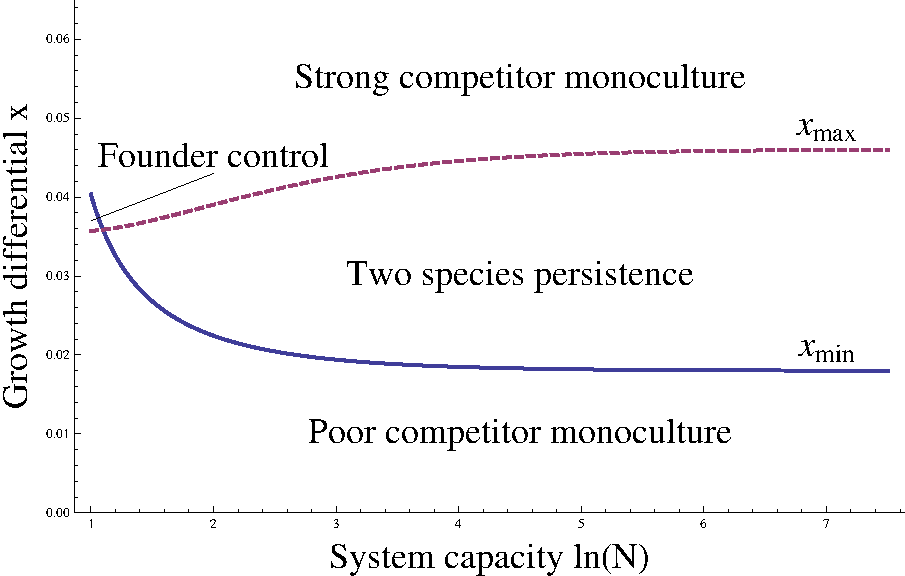
\includegraphics[width=4.5in]{xrangeofcoexist}
   \caption[Range of parameters giving coexistence without disturbance]{The effects of system capacity $N$ on the range of $x$ that will promote coexistence in the fecundity-growth trade-off model without disturbance. Should $x$ be too large, the more fecund species will likely be driven to extinction, while if the growth rates are very similar and $x$ drops below the lower limit then the more fecund species will competitively exclude the other species. When $x_{min}>x_{max}$ at low $N$, founder control occurs. Parameter values are $s_1=500,s_2=50$.}
 \label{fig:systemsize}
\end{figure}

When productivity is altered the effects depend on how productivity is implemented. Productivity, the production rate of new biomass, can be in the form of increased seed numbers (fecundity) or by increased juvenile growth rate. If juvenile growth rates are altered by a factor $\zeta$ for both species, then the effect is to alter the time $x$ for which species 2 can succeed with a secondary invasion by a factor $1/\zeta$, such that, for example, a doubling of juvenile growth rates halves the time species 1 juveniles spend vulnerable to competition.  In contrast, the effect of increased (or decreased) seed numbers by a factor $\phi$, with each individual therefore producing $\phi s_i$ seeds, is to increase (or decrease) the magnitude of the exponential term in $P(increase(n))$ and $P(decrease(n))$ by a factor $\phi$. This is equivalent to increasing (or decreasing) the time $x$ for which `invasion' is possible by the same factor. Note that if both growth rates and seed numbers vary with productivity the effective value of $x$ will be altered by a factor $\phi / \zeta$.

One further way that productivity can vary is if not all individuals are reproductively active at a given moment in time. Studies have demonstrated that the proportion of individuals producing seeds can vary widely, even over small spatial scales (REF!). To model this, we assume that each individual produces seeds within a time step with probability $p$. We show in Appendix~\ref{app2c} that reducing productivity in this way results in a new coexistence range
\begin{equation}
\label{xrangep}
\frac{N\ln \left( \frac{p^2 s_1(N-1)(N-2)}{((N-1)p-1)(ps_1(N-2)+s_2)} \right)}{s_2}<x<\frac{\ln \left( \frac{(N-1)ps_1}{s_1+ps_2(N-2)}\right) N}{ps_2(N-2)}.
\end{equation}
which asymptotes to
\begin{equation}
\frac{1}{p}\left(\frac{1}{s_2}-\frac{1}{s_1}\right)<x<\frac{\ln\left(\frac{s_1}{s_2}\right)}{ps_2}
\end{equation}
as system capacity $N$ tends to infinity. This has two notable effects \textbf{as system capacity increases}. First, as when individual seed values are reduced ($\phi<1$), the values for $x_{min},x_{max}$ are increased (by a factor $1/p$). \textbf{The result of this increase is that larger differences in growth rates between species can give coexistence, when compared to the coexistence range when $p=1$. Second, $x_{min}$ as given by \eqref{xrangep} has an asymptote at $N=1/p$, where the value of $x_{min}$ is infinite.} Since coexistence requires $x>x_{min}$, coexistence cannot occur on average for systems with capacity smaller than the threshold $N=1/p$. Therefore, as $p$ decreases, and less individuals produce seeds at a given time, larger systems are required to get coexistence of both species as shown in Figure~\ref{fig:pnondist}.  
\begin{figure}[th]
\centering
   \begin{tabular}{rrrr}
   (a)&&(b)&\\
  &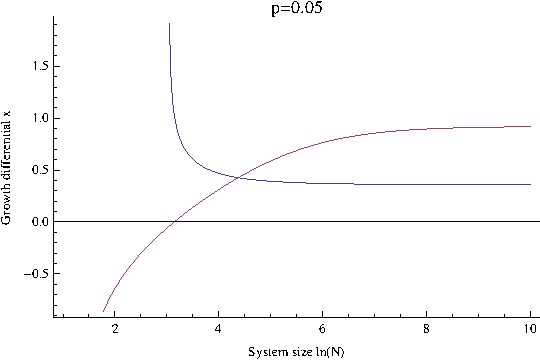
\includegraphics[width=2.5in]{p005nondist.pdf} && 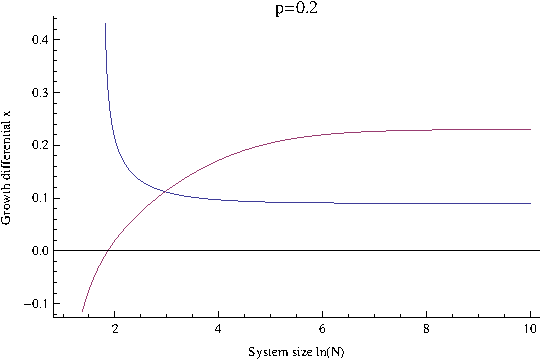
\includegraphics[width=2.5in]{p020nondist.pdf} \\
  (c)&&(d)&\\
  &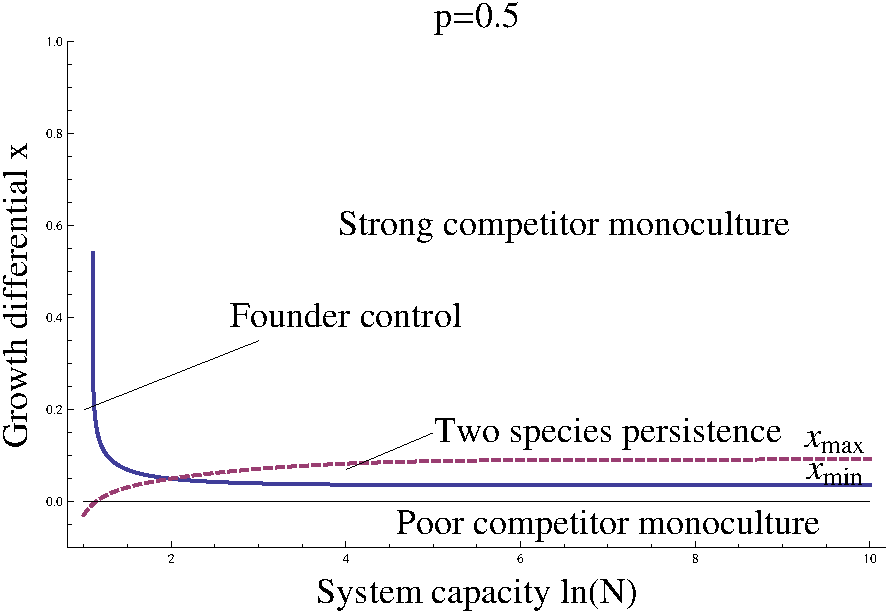
\includegraphics[width=2.5in]{p050nondist.pdf} && 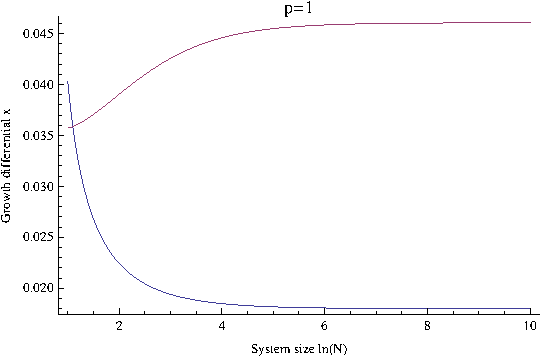
\includegraphics[width=2.5in]{p100nondist.pdf} \end{tabular}
   \caption[Coexistence without disturbance for reduced productivity]{The effects of altering the probability $p$ of an individual being reproductively active on the range of growth differential $x$ that gives coexistence, and how this varies with $N$, in an environment with no disturbance. Decreasing $p$ results in larger values of $x$ predicting coexistence, while simultaneously requiring larger system capacity $N$ to give this region of coexistence. Parameter values $s_1=500, s_2=50$.}
 \label{fig:pnondist}
\end{figure}


\subsection{The effects of disturbance events} \label{ss:resultsdist}
When disturbance events are introduced, there are three possible scenarios to study. First, when $x<x_{min}$, so that in the absence of disturbance the more fecund species 1 will exclude species 2, disturbance events cannot increase diversity by supporting the second species. Second, if the system can exhibit coexistence in the temporally homogeneous environment, moderate levels of disturbance (disturbance events with low intensity $I$ or very low frequency $f$) will retain this coexistence, with a shift in equilibrium abundances towards greater numbers of the more fecund species (results not shown). However, large intensities with intermediate or high frequencies will lead to a loss of diversity, creating a monotonically decreasing DDR, as species 1 will competitively exclude the less fecund species 2. \textbf{The third scenario is more interesting: when $x>x_{max}$, where in the absence of disturbance, the stronger competitor will competitively exclude the more fecund species}. Then it is possible that disturbance can promote coexistence. If the IDH holds, we would expect to see the species richness to increase then decrease as the size of disturbances is increased. Substituting the functions \eqref{increase}, \eqref{decrease} and \eqref{sp1} into the function given by \eqref{avchange} we can plot the region of $f-I$ parameter space that satisfies \eqref{ac1} and \eqref{acn-1}, revealing a region where long term coexistence occurs (Figure~\ref{hockey}).  The boundary of this region is where approximately half the simulations \textbf{are expected to exhibit coexistence}. In Appendix~\ref{app2d} we examine how time series simulations match the predictions given by using the approximation given by \eqref{avchange}, and note that for high intensity disturbances, the approximation becomes less accurate (see also Appendix~\ref{app2a}). When intensity $I=1$, at the first disturbance event, all individuals die, and so neither species \textbf{survives in the environment, and coexistence does not occur}. \textbf{However, in evaluating the expected change, the function is weighted towards non disturbance events when frequency $f$ is low. This can lead to an underestimation of the effects of high intensity disturbance events, and predict coexistence for parameters where the death of both species is inevitable.}
 Outside of this region with very high intensity, the approximation accurately captures the behaviour of simulations.

\begin{figure}[th]
\centering
  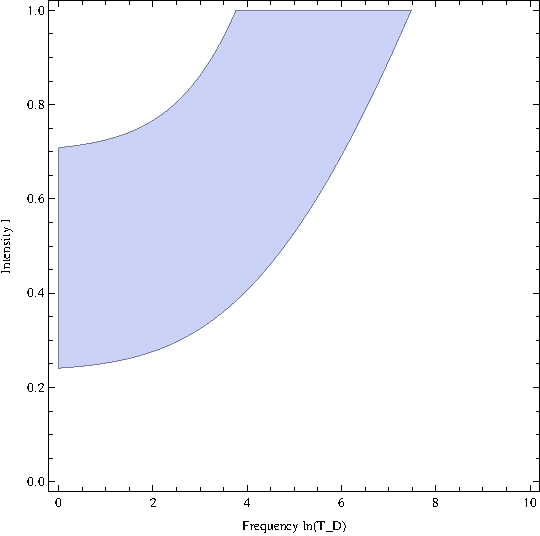
\includegraphics[width=5in]{hockeyTd.pdf}
   \caption[Coexistence with disturbance]{The region of coexistence (shaded area) for $x>x_{max}$ when $p=1$, and all individuals produce seeds within every event time step. Changes in disturbance frequency or intensity can produce different DDRs, with the humped, unimodal DDR predicted by the IDH one of several possible outcomes. Parameter values (a) $s_1=500, s_2=50, x=0.06,N=1000$.}
 \label{hockey}
\end{figure}

Analysis shows that it is possible to get very differently shaped DDR curves in this model, and this is affected by which factor influencing disturbance is considered. Increasing intensity can give very different responses to altering the frequency of disturbances. If $f=(dNT_D)^{-1}$ is fixed such that $1/f<T$, where $T$ is the expected time to extinction (see Appendix~\ref{app2b}), increasing intensity will give a humped DDR. \textbf{For example, if $\ln(T_D)=1$ is fixed in Figure~\ref{hockey}, and intensity increased from $I=0.1$, we initially see an increase in diversity as intensity crosses the point $I\approx0.25$. As intensity is increased further, however, there is a decline in diversity at $I\approx0.72$. This produces the classic peaked DDR predicted by the IDH.} 

However, if the fixed frequency is low, coexistence is impossible for any intensity $I$, and so a flat DDR is produced. Meanwhile, if intensity $I$ is fixed, while frequency of disturbance is varied, there are three possible scenarios: i) When $I$ is low \textbf{(e.g. $I=0.1$), the stronger competitor, species 2, will dominate regardless of frequency; ii) For intermediate intensities (e.g. $I=0.5$), increasing frequency will cause diversity to increase from one species to two (when $\ln(T_D)\approx 5$ for $I=0.5$), a monotonically increasing DDR; iii) When intensity is high (e.g $I=0.8$), increasing frequency will match the predictions of the IDH, giving a peaked DDR with coexistence occurring for intermediate frequencies (when $I=0.8$, the peak in diversity is predicted in the range $2\leq \ln(T_D) \leq 6$).} However, this coexistence occurs for a narrow range of $f$ (Figure~\ref{fig:simulationdata} in Appendix~\ref{app2d}). 

Increasing system capacity has a similar effect as in the non disturbance case, where increasing systems size can increase the range of parameters that give coexistence slightly, but the region of coexistence asymptotes quickly to a fixed region of parameter space as $N$ increases. This is caused by a stabilisation of the relationship between the dominant eigenvalue that determines the speed of community dynamics, and the number of events that occur in a fixed time period. With a fixed death rate (here 1\% per year), the number of events that occur per year in the present model scales linearly with system capacity, such that in a forest twice as large, we can expect to observe twice as many death events each year. As shown in Appendix~\ref{app2b}, the eigenvalue that determines the pace of the dynamics, and thus the time to converge to either the boundary or the internal quasi-equilibrium, asymptotes in a non linear fashion to $1$. For small systems ($N<300$), an increase in system size will have an exponential effect on increasing the time to extinction. This extended time to extinction increases the likelihood of an infrequent disturbance event occurring before extinction. In other words, a long transient towards a community dominated by a competitively dominant (e.g. shade-tolerant, late-successional) species will enable a shade-intolerant, pioneer species to be maintained before the next disturbance event shifts the environment into its favour. Once $N$ increases above a certain value, the change in time to extinction as a function of system capacity can be approximated by a linear relationship. Thus, owing to this linear relationship, while the time to extinction (measured in events) doubles as system capacity is doubled, the same change occurs in how many events are expected to occur. Therefore, the disturbance frequencies that give coexistence (for a given intensity) remain unchanged as system capacity increases further. This ensures that the systems response to disturbance regimes is robust to changes in system capacity.

These results are also robust to changes in productivity. A decrease in growth rates or increase in average seed production (such that $\phi/\zeta>1$) will shift the values of $x$ that give coexistence without disturbance to lower values. This in turn causes a shift in the disturbance intensities $I$ that give coexistence for a fixed $x$. If $x \in (x_{min},x_{max})$, this change in productivity can cause the value of $x_{max}$ to move below $x$, which means that low intensity disturbances may no longer  give coexistence. If species 2 excludes specie 1 in the absence of disturbance, increasing $\phi/ \zeta$ will move the diversity peak where both species coexist to higher disturbance intensities, matching the predictions of dynamic equilibrium models (Huston 1979; Kondoh 2001). In contrast, reducing $\phi/\zeta$ by increasing growth rates or decreasing seed production will increase the values of $x$ for which coexistence occurs without disturbance (as determined by \eqref{xrangep}).This has the effect of lowering the intensities for which coexistence can occur.

However, while a change in productivity can \textbf{alter the range of disturbance regimes for which coexistence occurs for a given set of parameters, the qualitative results do not change.} Using an approximation for the expected change when individuals are reproductive with probability $p<1$(outlined in Appendix~\ref{app2e}) it is possible to see that when seed production in decreased, the results are qualitatively similar, displaying a `hockey stick' type shape to the coexistence region (Figure~\ref{pfigure}). \textbf{Figure~\ref{pfigure} also shows how reducing $p$ has similar effects to a reduction in the value of $x$}. While the asymptote to a fixed region as $N$ increases is slightly slower when $p$ is reduced, coexistence still asymptotes to a fixed region as we increase system capacity, demonstrating that these results are robust to changes in both productivity and system capacity.

\begin{figure}[htbp]
\begin{center}
\begin{tabular}{cccc}
(a)&&(b)&\\
&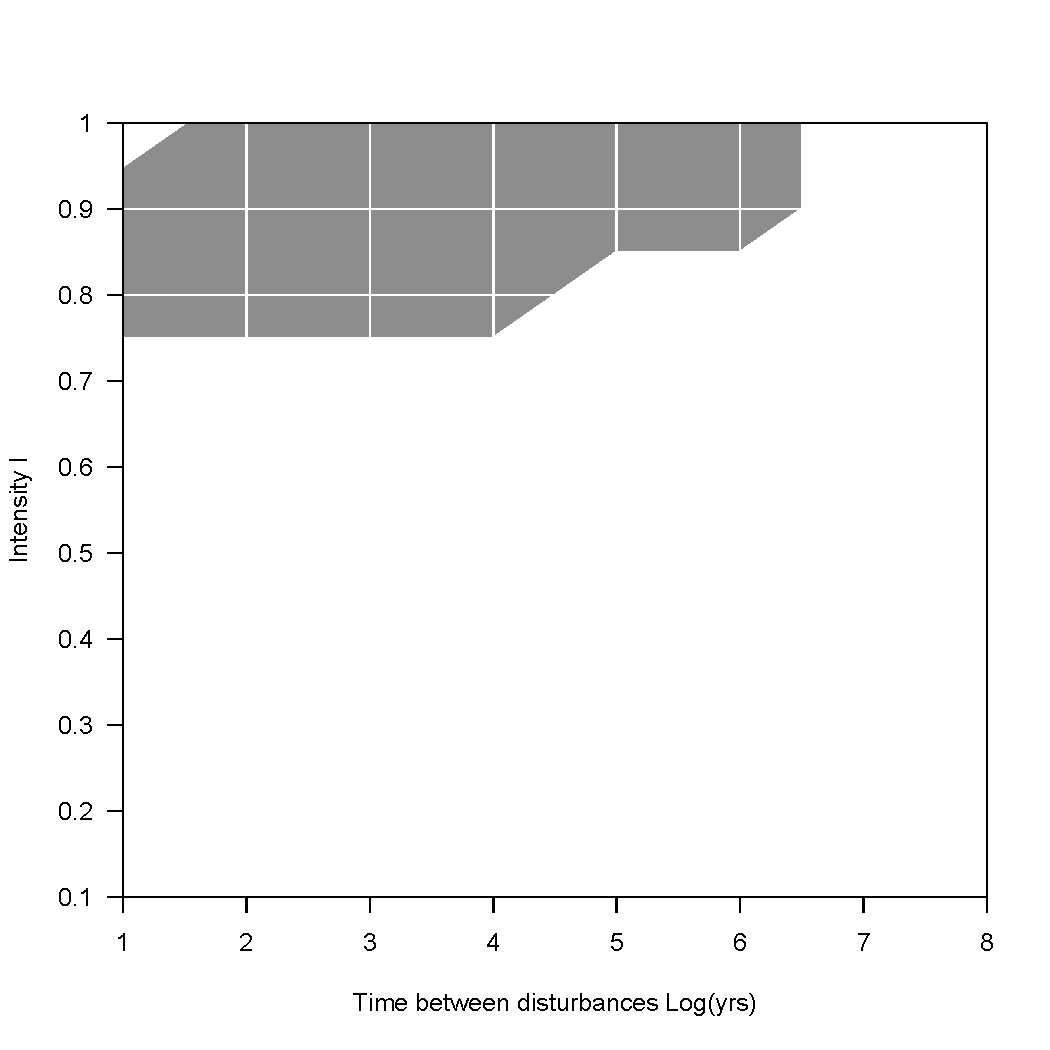
\includegraphics[width=2.5in]{pplot75.pdf} &&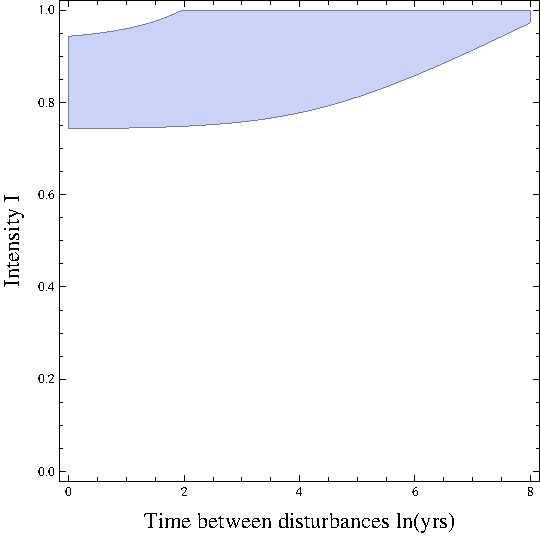
\includegraphics[width=2.5in]{p0p75xequiv.pdf}\\
(c)&&(d)&\\
&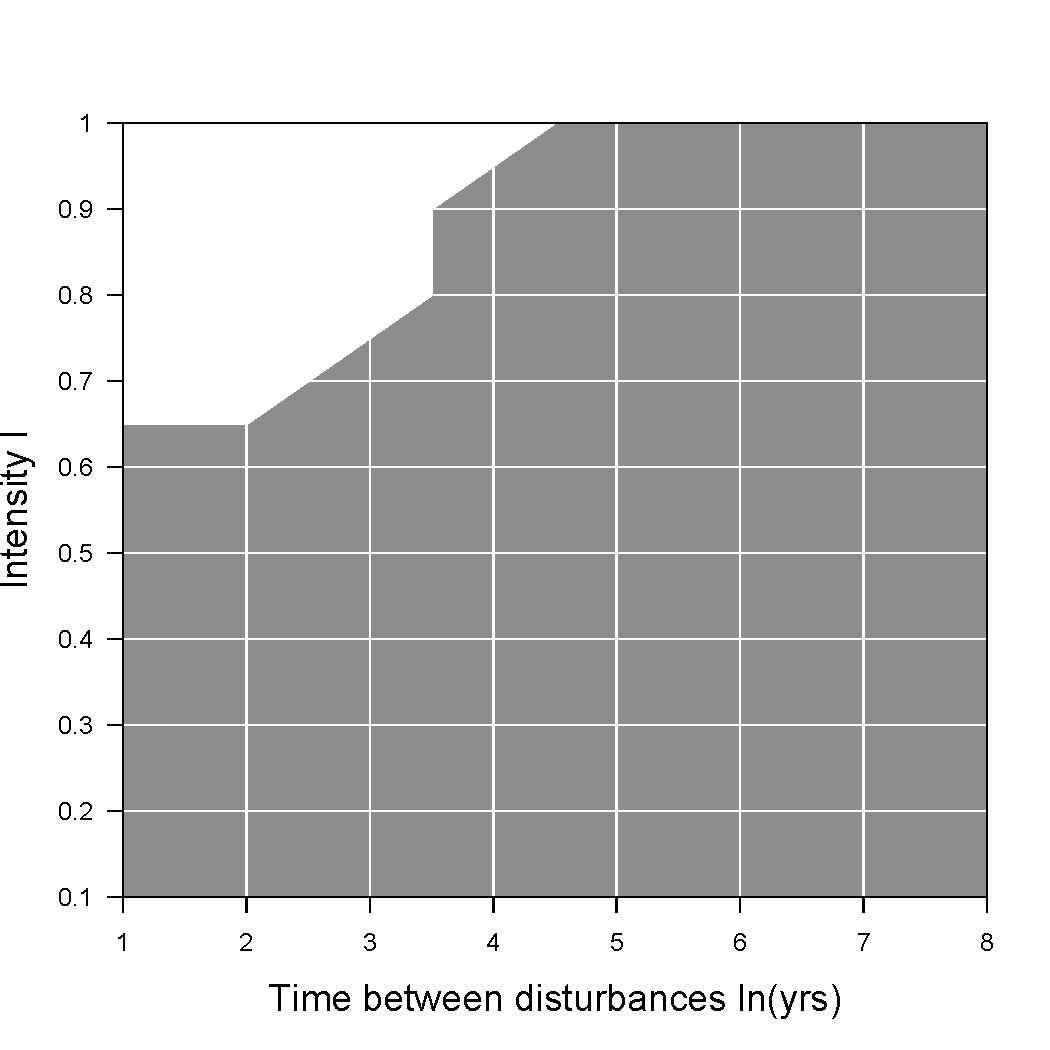
\includegraphics[width=2.5in]{pplot10.pdf} &&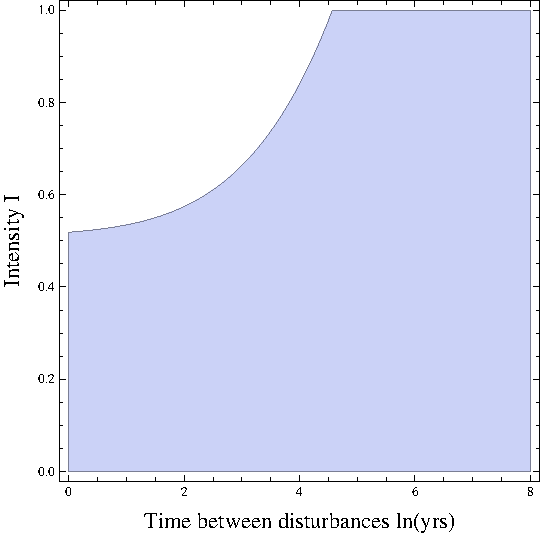
\includegraphics[width=2.5in]{p0p2xequiv.pdf} \end{tabular}
\caption[Coexistence with disturbance for reduced productivity]{The effect of reducing the probability of an individual being reproductively active $p$ on the disturbance regimes that predict coexistence. Reducing $p$ has a similar effect as transforming the growth rate differential $x \to px$. Shaded areas are where coexistence is predicted. (a) and (c) show the region of predicted coexistence using the approximation given in Appendix~\ref{app2e} for $s_1=500,s_2=10,x=2$ for (a) $p=0.75$ and (c) $p=0.1$. The approximation is evaluated at $\ln(T_D)=i, I=0.1j$ for alll $i\leq8, j\leq 10$, and a linear extrapolation used between points (b) and (d) illustrate that the effect is the same as reducing $x$ to (b) $x=1.5$ and (d) $x=0.2$. Note that $x_{max}=\ln(500/10)/10\approx 0.39$, such that (c) and (d) represent parameters where coexistence occurs in the absence of disturbance.}
\label{pfigure}
\end{center}
\end{figure}


\section{Discussion} \label{discuss}
Disturbance is often considered an important driver of biodiversity and species richness \citep[e.g.][]{denslow1987tropical,lawton1988natural,sousa1984role}. We use a lottery type model to confirm that while it is possible for two species to coexist along a fecundity-growth trade-off in a homogeneous environment, disturbance events can dramatically increase the range of parameters for which coexistence is possible. Analysis shows, in accordance with recent theory \citep{miller2011frequency}, that different factors influencing disturbance (here frequency or intensity) can have very different effects, and may impact species richness in different ways. We add to this theory by determining analytic conditions for coexistence under given disturbance regimes, and by demonstrating that these conditions are robust to model type, productivity and system size. We suggest these general results may explain in part some of the conflicting empirical results regarding the IDH. Indeed, one consequence of our results is that it is possible for two forest fragments to \textbf{exhibit different diversity patterns, even though all species in both sites have the same vital rates (i.e. same seed productivity and growth rates). Further, an increase in either disturbance frequency or intensity can have different effects, and these effects are dependent on the underlying disturbance regime. For example, a region with infrequent disturbances of intermediate intensity may show an increase in diversity as disturbances become more frequent, while a different forest with more frequent yet less intense disturbances may not exhibit this increase in diversity with frequency.}

In general, our results indicate that it is important to consider the intensity and frequency of disturbance events as separate parameters when studying the effects of disturbance on diversity levels, and emphasise that past disturbances can have long-lasting effects, which persist for decades or centuries, in accordance with \cite{foster1999human}. \textbf{In the current model, these effects come in the form of persistence of inferior competitor species, which can be sustained for many time steps between disturbances as infrequently as every 400 years. The result here is} increased diversity within the canopy, but disturbance can effect several other aspects of the environment, such as net primary production \citep[e.g.][]{turner2010disturbance}. These results, while arising in a new model, are qualitatively similar to those of \cite{miller2011frequency}, adding weight to the suggestion that the separation of factors controlling disturbance is an important consideration in studying the effects of disturbance on a community. We build on this work by showing that these qualitative results are extremely robust to parameter changes.

\textbf{Our results also demonstrate that frequency and intensity can have different effects across a broad range of system capacities and productivity levels. The model reproduces the results of \cite{kondoh2001unifying} when disturbance frequencies are high, showing a diversity peak at lower disturbance intensities  when productivity is reduced. The current model also finds that disturbance regimes that maximise coexistence may be predicted by a combination of system productivity and the life histories of species in the community. However, these results are not applicable to alternative measures of disturbance. For example in the current model a moderate change in productivity has negligible effect on the community response to increased frequency. The current model here demonstrates that the results of Kondoh are not universal, further emphasising the importance of considering different factors determining disturbance.}

Many plant populations are thought to be recruit limited \citep[e.g.][]{clark1998stages,eriksson1992seed,svenning2005seed}, and this may be particularly important in very species rich communities, where most species are locally quite rare \citep[e.g.][]{svenning2005seed}. By relaxing the assumption that all individuals are reproductively active at the time of the disturbance, or otherwise altering the seed production in the system, we also show the importance of seed limitation on the community dynamics. Our analyses show that seed limitation generally increases difference in growth rates \textbf{that allow species to coexist}, and this is in line with previous theory that shows recruit limitation often slows dynamics, especially in species rich communities \citep{hurtt1995consequences}. This again suggests that processes that slow down the dynamics will act to help support the maintenance of competitively weaker (e.g. pioneer) species. \textbf{While modelling sexual (non-selfing) species would require a different analysis, sexual species may experience slower dynamics because they become both pollen and seed limited with pollen limitation leading to reproductively active trees not bearing fruit. The consequences of sexuality in this context remain an open question, and a more detailed model approach may be necessary.}

Another aspect in which our results differ from those of  \cite{miller2011frequency} is that at very high frequencies, their model exhibited a tailing off of coexistence \citep[Figure 1 of ][]{miller2011frequency}, resulting in a crescent shaped region of coexistence. Our model does not  present this tailing off, and even when $f=1$, a relatively broad range of intensities can give coexistence. We suggest that this is because our model allows for full site replenishment following a disturbance event before a second disturbance is possible. Our assumption makes the model computationally much simpler, at the expense of some realism. However, the assumption of full replenishment will only alter outcomes at very high intensities, where very few individuals survive. In the case where at least 2\% of the system survives a disturbance event, this would allow for complete replenishment, on average, between very common disturbance events, such as El Nino, which strikes with a frequency of approximately once every 5 years. When the system considered is shrub- or grassland, we anticipate that site replenishment will also be rapid.

While we only consider two species in the current model, previous work has argued that disturbances may enhance coexistence i multi-species communities \citep[e.g.][]{loehle2000strategy,roxburgh2004intermediate}. Earlier theory has suggested that infinitely many species can coexist along a spatially implicit competition-colonisation trade-off \citep[e.g.][]{tilman1994competition}, and that spatial structure is not necessary for generating large numbers of species \citep{adler2000space} although for large numbers of species coexistence is highly unlikely \citep[Chapter~1;][]{nattrass2012quantifying}. \textbf{Further, \cite{gyllenberg2005impossibility} show that the coexistence of infinitely many species is structurally unstable. Chapter 4 of this thesis considers} models featuring greater species numbers, which we anticipate will produce qualitatively similar results, with many different diversity curve shapes generated by different combinations of frequency and intensity, even when the overall biomass loss due to disturbance is identical. The key element to generating coexistence is that no one species is superior across the entire range of disturbance gradient, and this means further underlying niche differences are required in order to support higher number of species \citep[e.g.][]{seifan2013beyond}. Nonetheless, comparisons of different forests with different levels of disturbance frequency and intensity do exist. For example, \cite{denslow1987tropical} reports on two forests, one in Puerto Rico which has not experienced any hurricanes in the last 150 years, and one in Costa Rica which experiences a hurricane once every 20-30 years. Despite having otherwise similar annual rainfall and topology, the former site supports only 88 tree species in 16ha of study plots, whereas the latter supports 269 species in 12.4ha of plots. Although other differences are apparent, such as the amount of human activity and isolation from the mainland, the Costa Rican forest does have a faster turnover of trees caused by tree fall and the theory presented here does predict forest with the more frequent but less intense disturbances to have the fewer species.

The current model does not include spatial heterogeneity. Previous studies suggest that spatial structure does not have a significant effect of disturbance events and their aftermath in a number of circumstances, such as when the disturbance does not have directionality \citep{frelich1991natural}. However, given that most seeds of most plants fall near to the parent, incorporating realistic dispersal kernels could influence the relative importance of disturbance to the community dynamics. Many plant communities show within-species clustering, meaning nearby neighbours are quite likely to be conspecifics \citep{condit2000spatial,murrell2001uniting}, and deaths of individuals leave gaps that most likely to be exploited by these neighbours. Generally speaking it is expected that such localised dispersal should slow down the community dynamics both in terms of time to expected exclusion (Gandhi et al. 1998) and also potentially during the invasion process \citep{murrell2010does}. Which of these two effects dominates remains an open question for the model presented here, and metapopulation theory suggests the effect on the dynamics might be quite complex \citep{ovaskainen2002transient}. However, we suspect in many cases the effect of restricted dispersal on all species will help maintain the weaker competitor in the community because restricted dispersal will mean it can win some sites uncontested.

Often, disturbance is modelled using a single parameter, as reviewed by \cite{shea2004moving}, yet we demonstrate that identical overall disturbance rates can produce different environmental conditions, and different diversity levels. This extends to the consideration of diversity curves as disturbance is varied. The same change in overall disturbance levels can result in dramatically different diversity curves, with monotonic curves and both peaked and U-shaped curves, although the latter are difficult to achieve. These results are in accordance with the findings of \cite{mackey2001diversity}, who report that peaked and monotonic DDRs are all relatively frequent, while U-shaped curves are much rarer. The differences in effect on biodiversity between the factors governing the total level of disturbance could therefore suggest an explanation for the great variety of DDR shapes observed in nature. While we only consider two of these factors, frequency and intensity, we find that an increase in intensity will often give a humped DDR, while an increase in frequency of disturbance will present a monotonic or flat DDR, and this is robust to changes in all model parameters. Once other factors of disturbance are considered, a still broader range of DDR shapes may be explained by the variation of how disturbance is measured. Some recent empirical work has considered the effects of different disturbance measures \citep[e.g.][]{bertocci2005contrasting,collins1987interaction,svensson2009equal}, and the work presented here suggests that it should remain a point of emphasis for empirical studies.


\section*{Acknowledgements}
This project was funded by a National Environment Research Council studentship to Stuart Nattrass.

\section*{Appendices}

\bappendix
\section{Approximating the expected change function}
\label{app2a}
 When approximating the average change using the function given by \eqref{avchange}, we must compare these results to the actual expected change. Using the Law of Total Probability ($P(A)=\sum_{b \in B} P(A|b)P(b)$), \textbf{where $A$ is the probability of increasing species 1 numbers by $k$ individuals, and $B$ the set of possible death numbers in species 2, and summing the results weighted by $k$,} the average change at the boundaries is given by
\begin{align}
\label{acreal1}&AvCh(1)=\frac{-I+(N-1)I^{N-1}(1-I)}{dNT_D}\\
&+\frac{(1-I)\sum_{k=1}^{N-2}\sum_{j=k}^{N-2}k I^j(1-I)^{N-2-j}{N-2\choose j} Sp_1(1,N-1-j)^k(1-Sp_1(1,N-1-j))^{j-k} {j \choose k}}{dNT_D} \notag \\
 &+ \left(1-\frac{1}{dNT_D}\right)(P(\text{Increase}(1))-P(\text{Decrease}(1))), \notag \\
 \label{acrealtot}&AvCh(N-1)= \frac{-I^{N-1}(N-1) +I(1-I^{N-1})}{dNT_D} \\
 &-\frac{(1-I)\sum_{k=1}^{N-2}\sum_{j=k}^{N-2}k I^j(1-I)^{N-2-j}{N-2\choose j} Sp_1(1,N-1-j)^{j-k}(1-Sp_1(1,N-1-j))^{k} {j \choose k}}{dNT_D} \notag \\
 &+ \left(1-\frac{1}{dNT_D}\right)(P(\text{Increase}(N-1))-P(\text{Decrease}(N-1))). \notag
  \end{align}
where $Sp_1$ is as defined in \eqref{sp1}. Since these sums become computationally expensive for large system size, we approximate these using \eqref{avchange}. Figure~\ref{fig:approxerror1} shows how the error varies when \eqref{avchange} is used to approximate \eqref{acreal1}. The error of the approximations decreases with increased time between disturbances $T_D$, decreased intensity $I$, and increased system capacity, while Figure~\ref{fig:approxerrortot} shows the same effects of system size and disturbance frequency for approximating the average change when $N-1$ sites are occupied by species 1 given by \eqref{acrealtot}. However, in this case the relationship between error and intensity exhibits a peak in error size for intermediate intensities. \textbf{This may be because for the upper boundary condition \eqref{acrealtot}, the exponential term in \eqref{sp1} exhibits greater variation than in \eqref{acreal1}, and that this error is maximised at intermediate values of $I$. While only the errors generated by one set of parameters are shown in Figures~\ref{fig:approxerror1} and \ref{fig:approxerrortot}, the qualitative results are robust to parameter changes.}
 \begin{figure}[th]
\centering
   \begin{tabular}{rrrr}
   (a)&&(b)&\\
  &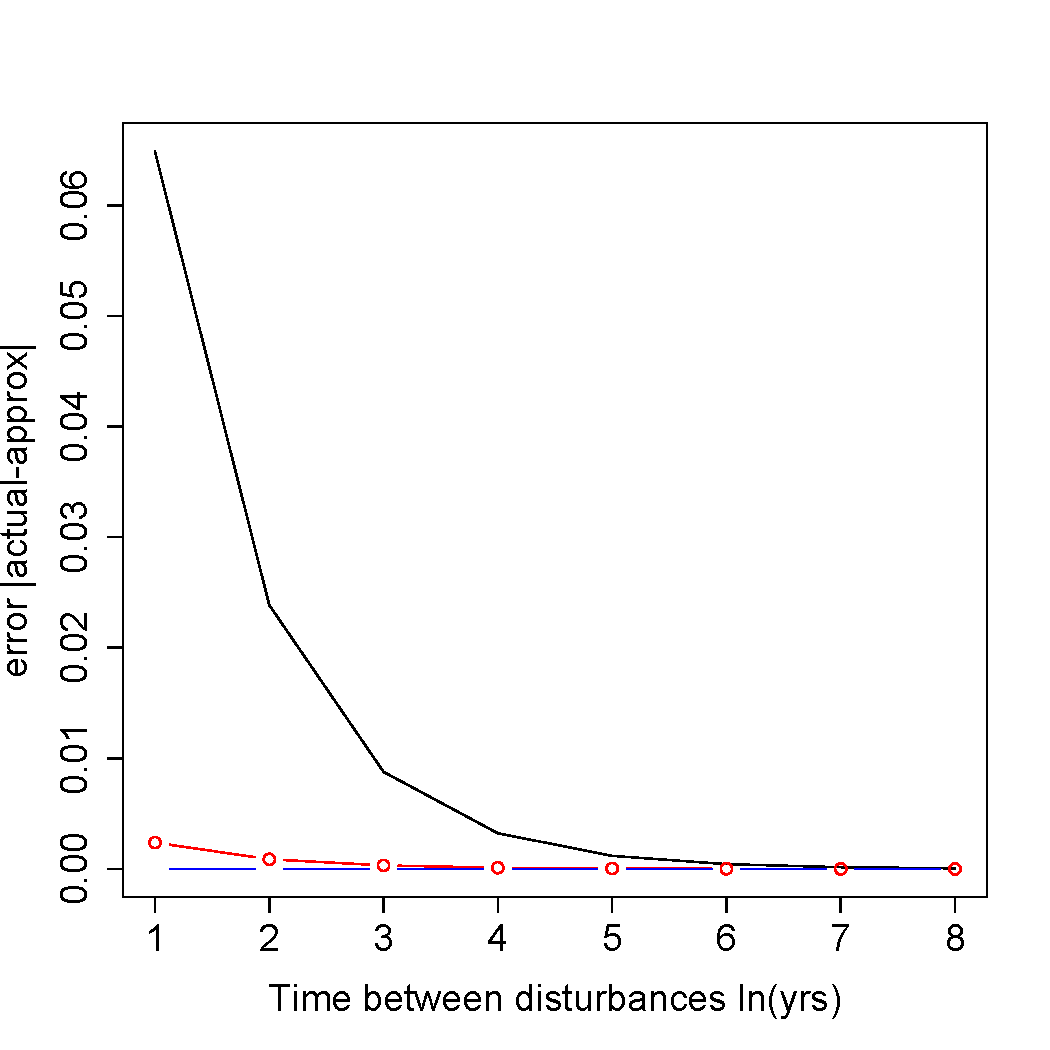
\includegraphics[width=2.5in]{errwithTlb.pdf} && 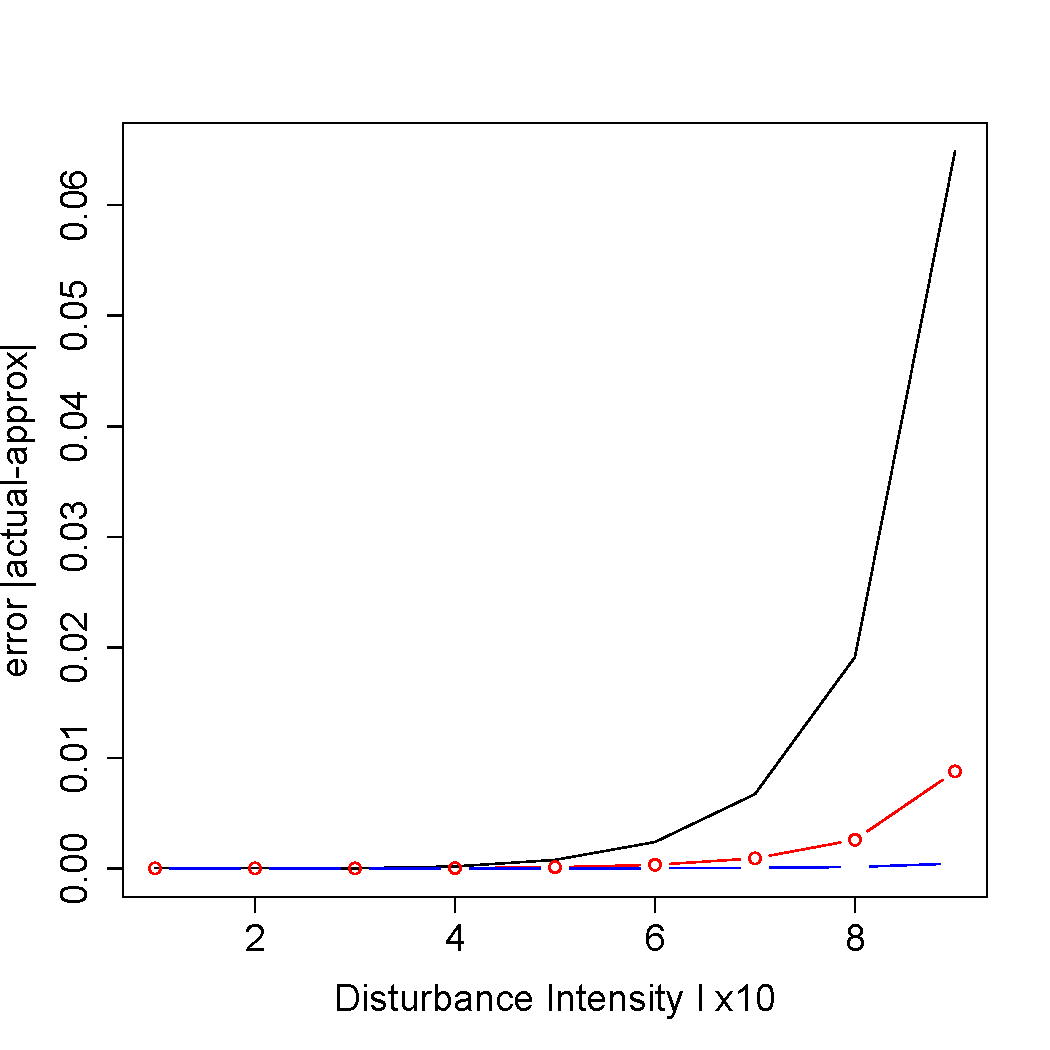
\includegraphics[width=2.5in]{errwithIlb.pdf} \\
  (c)&&(d)&\\
  &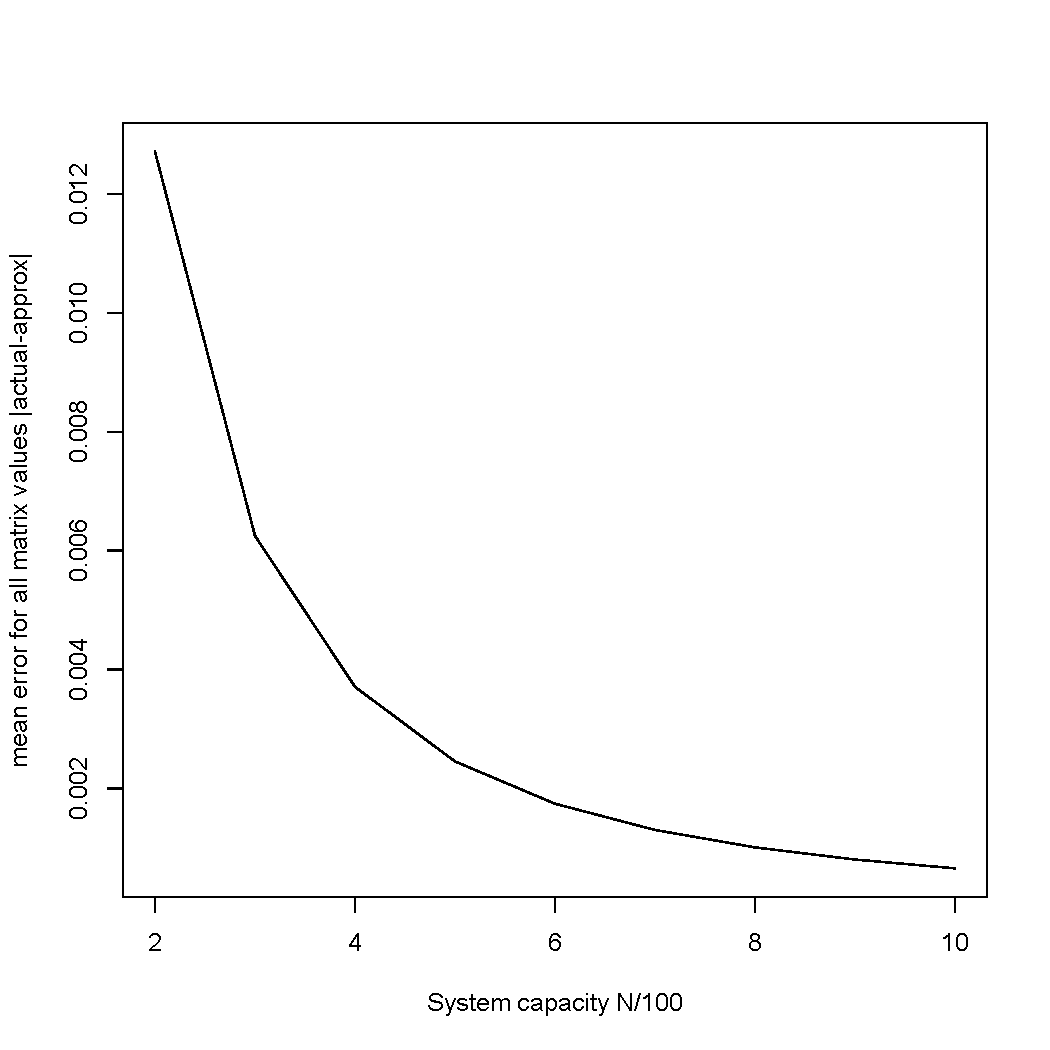
\includegraphics[width=2.5in]{meanerrorovermatrix.pdf} && 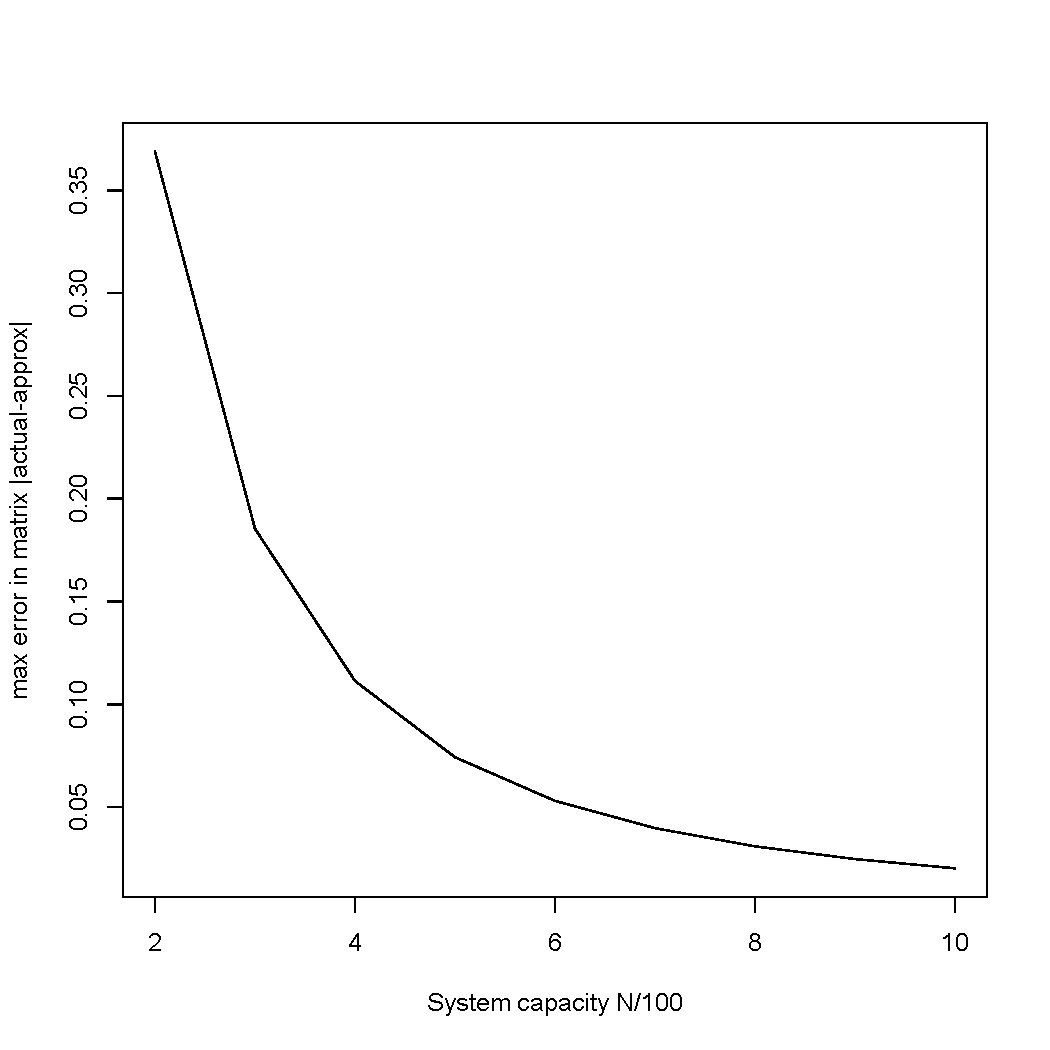
\includegraphics[width=2.5in]{maxerrorovermatrix.pdf} \end{tabular}
   \caption[Approximation errors for species 1 invasion]{(a) How the error of the approximating function for species 1 invasion changes with increased time between disturbances $T_D$ for various intensities $I=0.3$ (blue, dashed lines), $I=0.6$ (red, dashed lines with points), and $I=0.9$ (black, solid line) (b) the effects of increasing intensity $I$ for fixed frequency $\ln(T_D)=1$ (black, solid line), $\ln(T_D)=4$ (red, dashed line with points) and $\ln(T_D)=8$ (blue, dashed line).. Errors are larger for higher intensity, but decrease as the expected time between disturbances increases. (c-d) How the mean (c) and maximum (d) error size decrease with increased system capacity $N$. The error was calculated for intensities $I=0.1,0.2,0.3,...,0.9$ and time between disturbances $\ln(T_D)=1,2,3,...,8.$ Parameters used are $s_1=500,s_2=50,x=0.06,N=500$.}
 \label{fig:approxerror1}
\end{figure}
 \begin{figure}[th]
\centering
   \begin{tabular}{rrrr}
   (a)&&(b)&\\
  &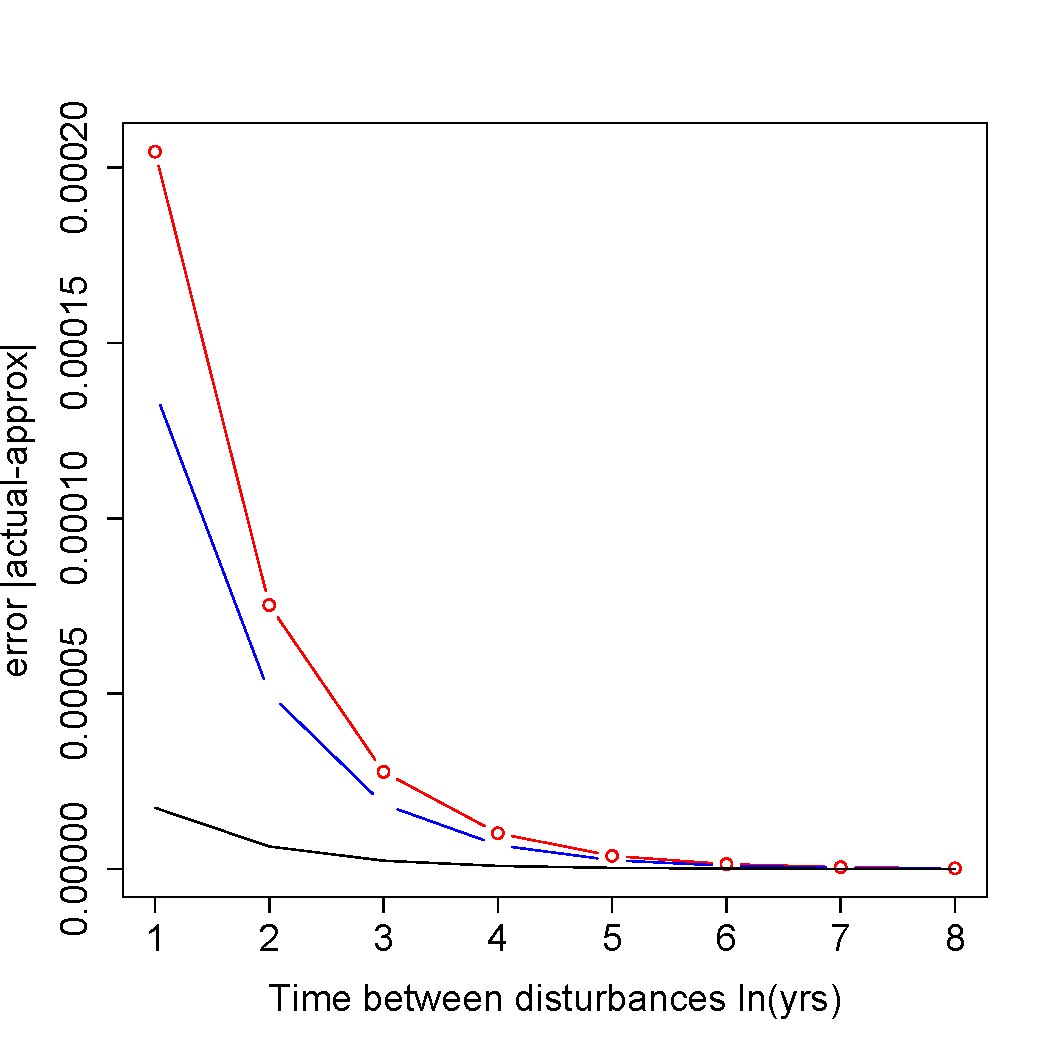
\includegraphics[width=2.5in]{errwithTub.pdf} && 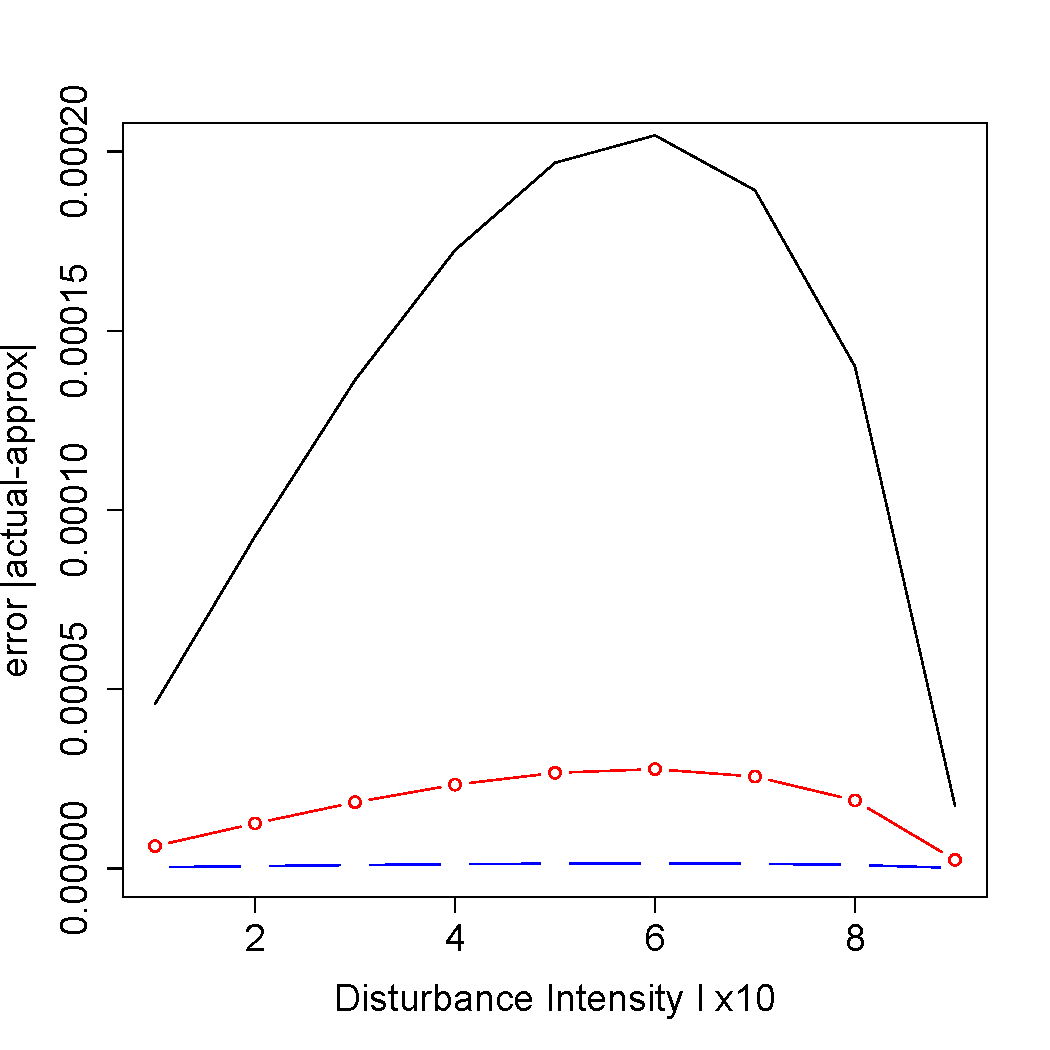
\includegraphics[width=2.5in]{errwithIub.pdf} \\
  (c)&&(d)&\\
  &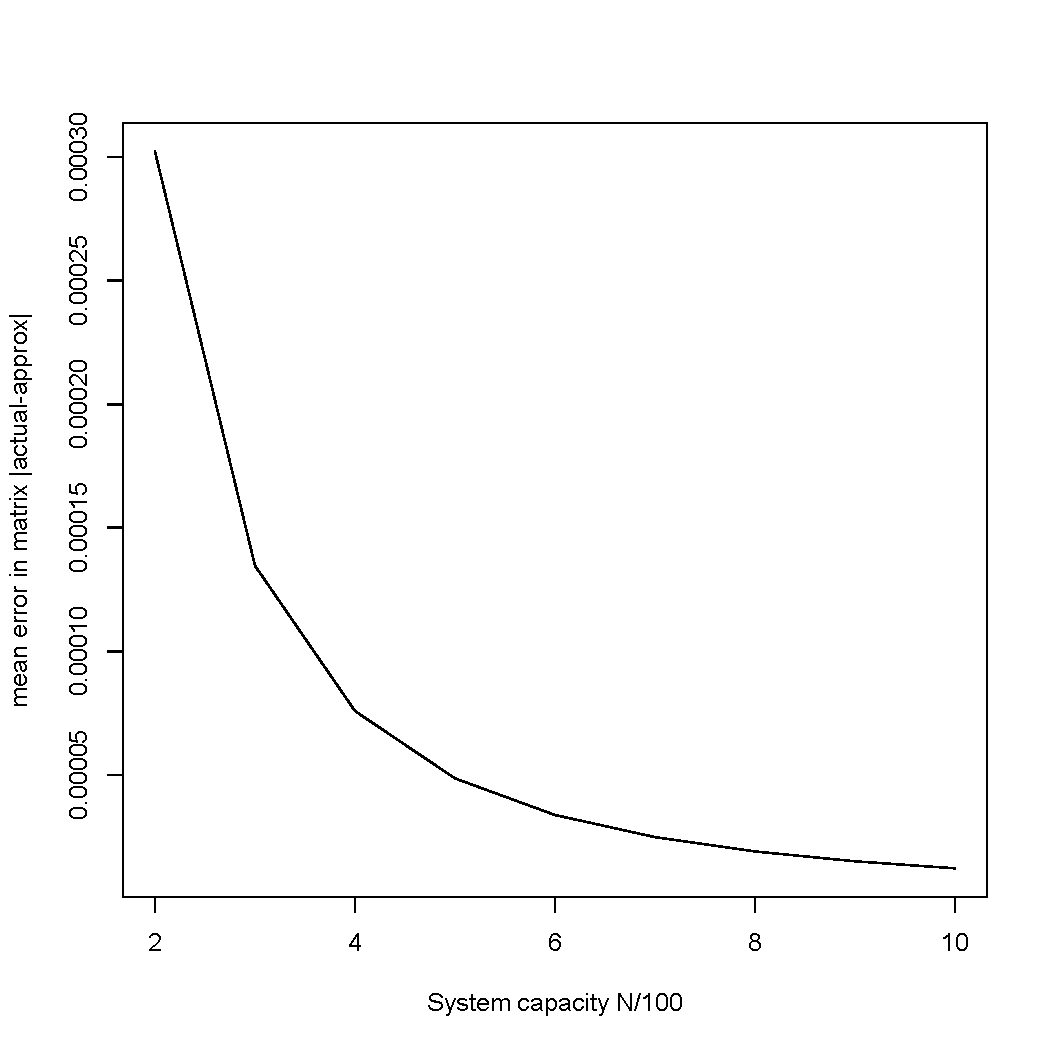
\includegraphics[width=2.5in]{meanerrortotovermatrix.pdf} && 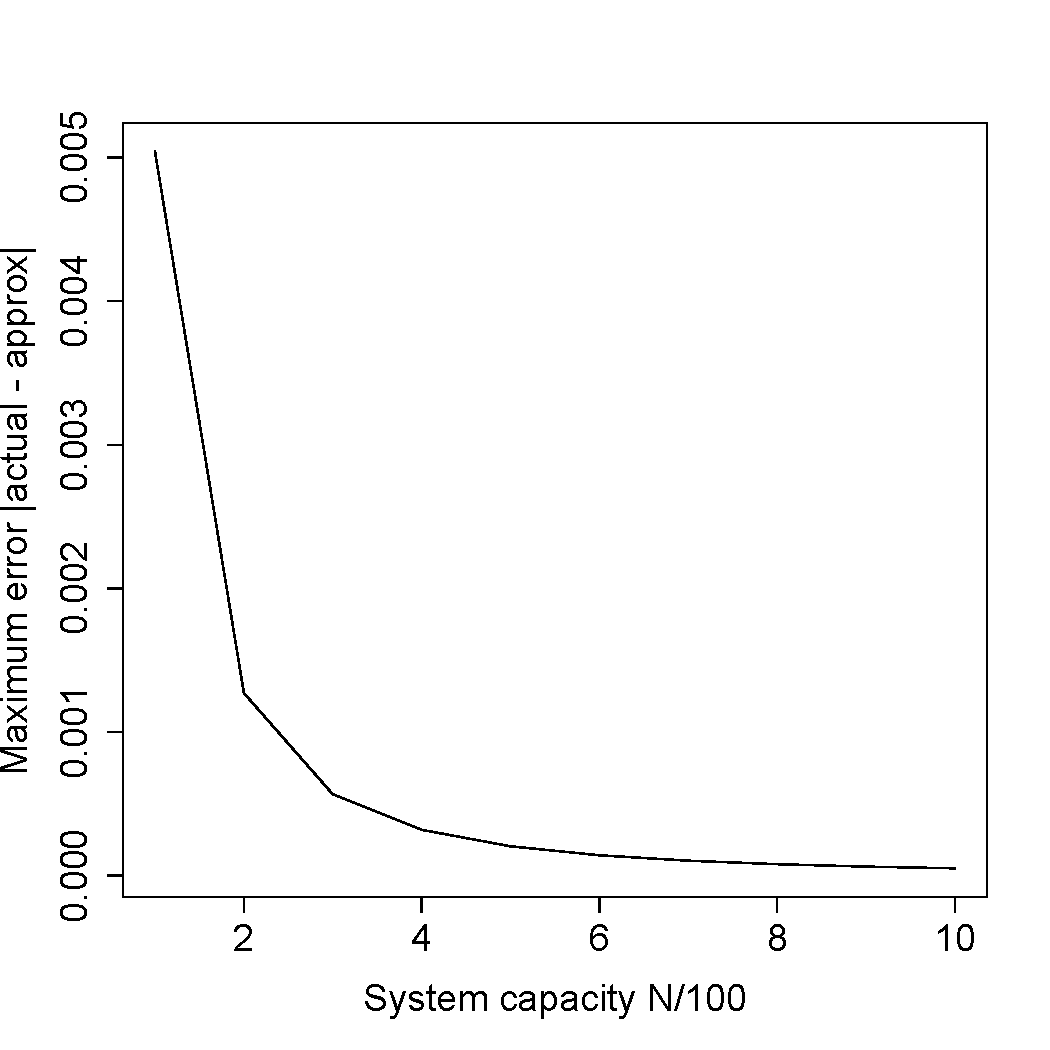
\includegraphics[width=2.5in]{maxerrortotovermatrix.pdf} \end{tabular}
   \caption[Approximation errors for species 2 invasion]{(a) How the error of the approximating function for species 1 invasion changes with increased time between disturbances $T_D$ for various intensities $I=0.3$ (blue, dashed lines), $I=0.6$ (red, dashed lines with points), and $I=0.9$ (black, solid line) , and (b) the effects of increasing intensity $I$ for fixed frequency $\ln(T_D)=1$ (black, solid line), $\ln(T_D)=4$ (red, dashed line with points) and $\ln(T_D)=8$ (blue, dashed line). Errors decrease as the expected time between disturbances increases, but display a non-monotonic relationship to intensity, with the largest errors produced by intermediate intensity. (c-d) How the mean (c) and maximum (d) error size decrease with increased system capacity $N$. The error was calculated for intensities $I=0.1,0.2,0.3,...,0.9$ and time between disturbances $\ln(T_D)=1,2,3,...,8.$ Parameters used are $s_1=500,s_2=50,x=0.06,N=500$.}
 \label{fig:approxerrortot}
\end{figure}


 \section{Expected time to convergence}
 \label{app2b}
 \begin{figure}[th]
 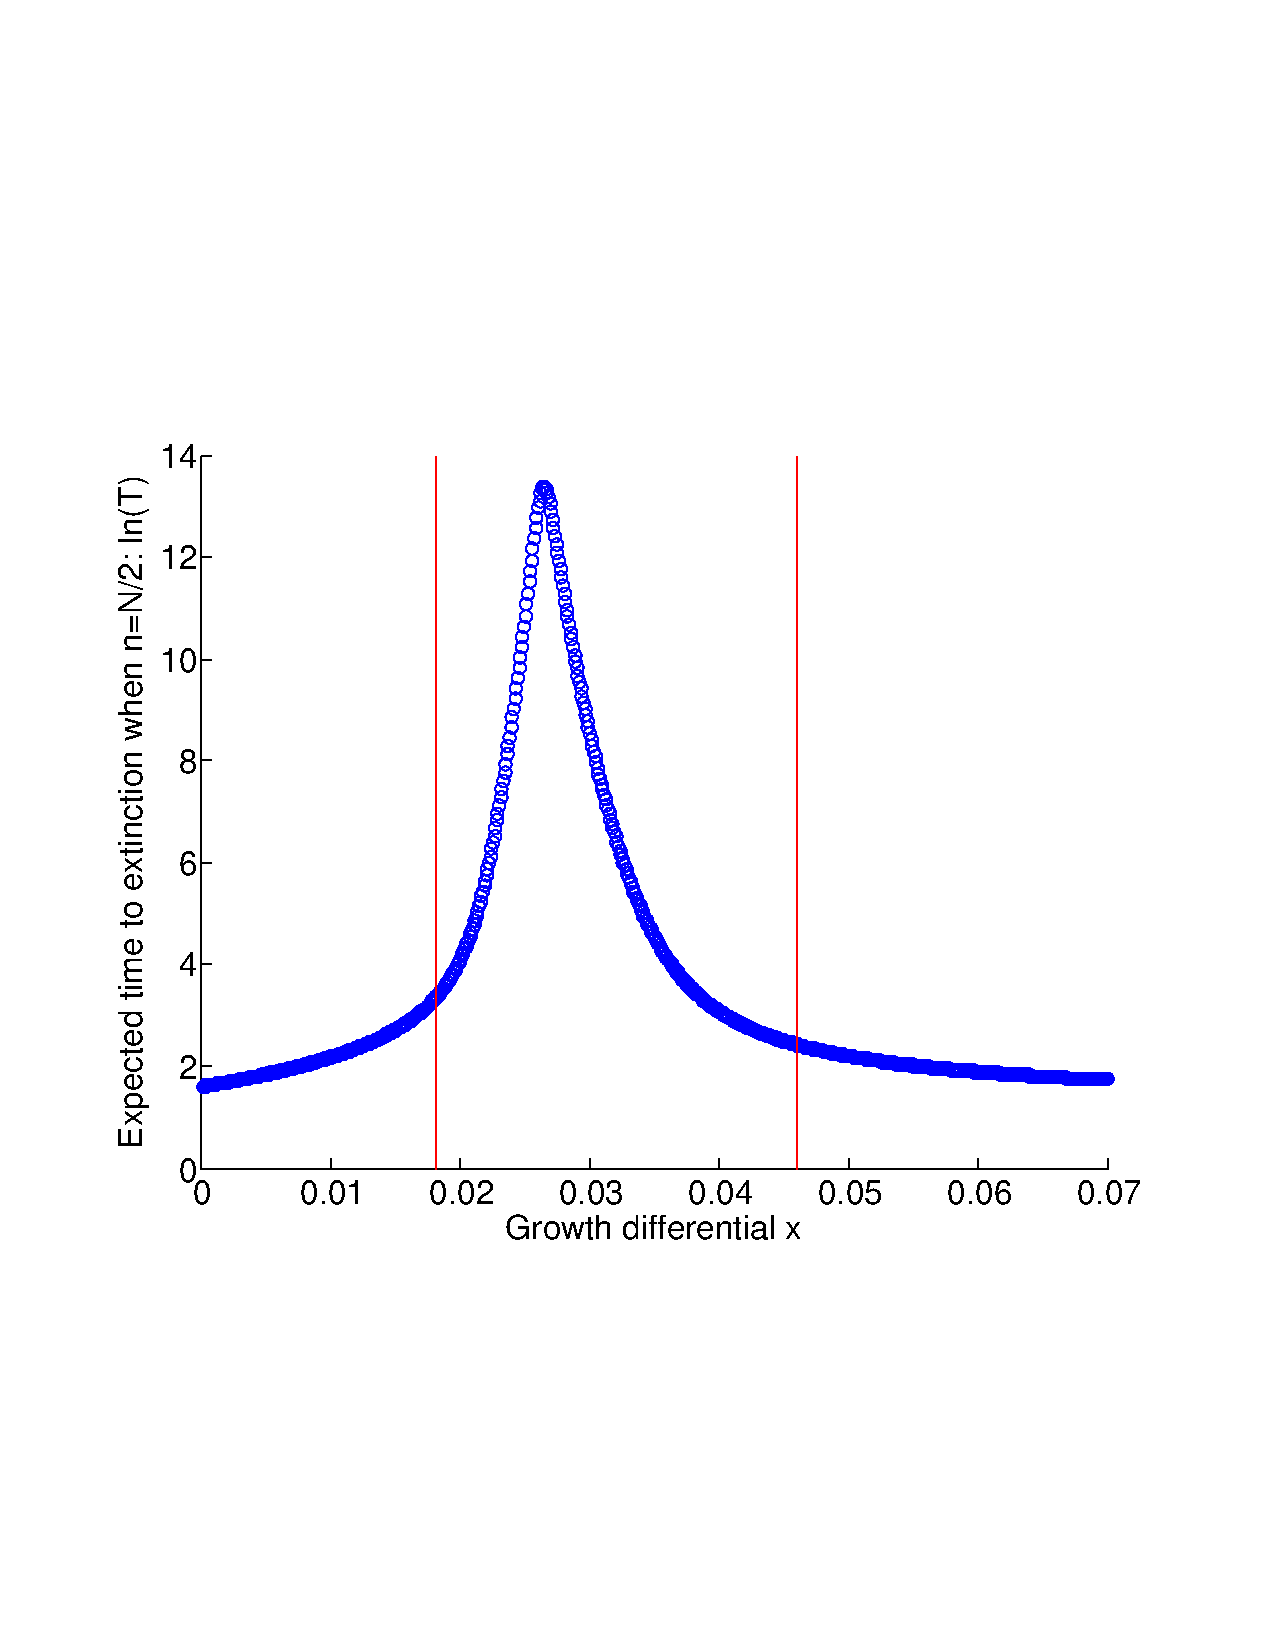
\includegraphics[width=4in]{ttevx.pdf}
 \caption[How time to extinction varies with the difference in growth rates]{The difference in growth rates as measured by time available for invasion $x$ effects the expected time to extinction, when measured from initial population $n=N/2$. Vertical lines represent $x_{min},x_{max}$, and the region predicted to give coexistence between these lines does display the highest expected time to extinction. Parameters are $s_1=500,s_2=50,N=100$.}
 \label{fig:ttevx}
 \end{figure}
 
 The expected time to extinction of the system can be calculated easily in the case where there is no disturbance. Defining the expected number of time steps taken to go from $n$ individuals of species 1 in an environment where disturbance does not occur to either of the absorbing boundaries ($n=0$ or $n=N$) as $k_n$, we can solve a series of simultaneous equations given by
\begin{equation}
k_n=\begin{cases}
0 & n\in\{0,N\} \\
1+P(\text{Increase}(n))k_{n+1}+P(\text{Stay}(n))k_n+P(\text{Decrease}(n)k_{n-1}) & 1\leq n\leq N-1
\end{cases} \end{equation}
to determine the vector $\mathbf{k}$ of expected extinction time for each possible initial population. This varies with growth rate differential $x$, as demonstrated in Figure~\ref{fig:ttevx}, yet also increases with system capacity $N$, as demonstrated in Figure~\ref{fig:tte}. As system size increases by an order of magnitude, the expected time to extinction increases by a greater ratio. This is especially the case within the range of $x$ that invasion analysis suggests gives two species coexistence. Here, increasing the system size from 100 to 1000 causes the expected time to extinction to increase by approximately 12 orders of magnitude.

\begin{figure}[th]
\centering
   \begin{tabular}{rr}
  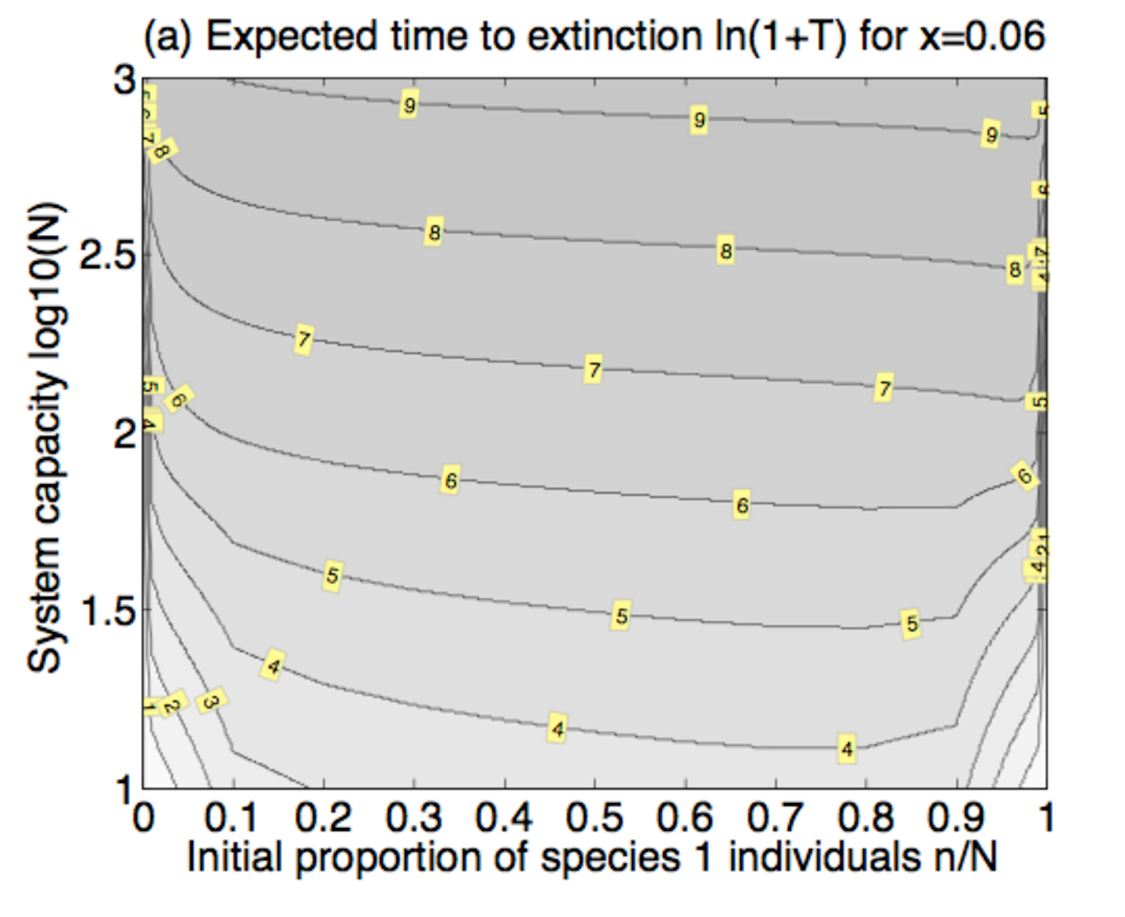
\includegraphics[width=2.5in]{x06resize.pdf} & 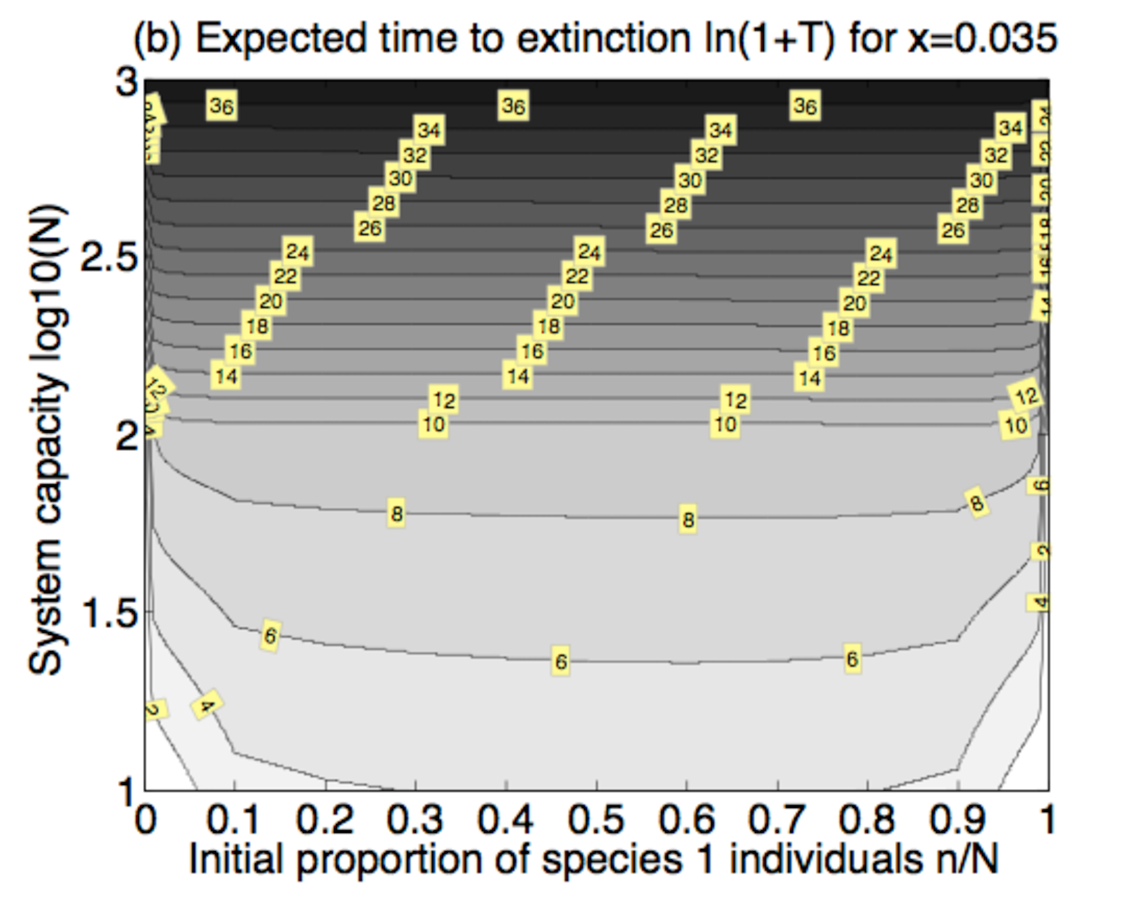
\includegraphics[width=2.5in]{x035resize.pdf} \\
  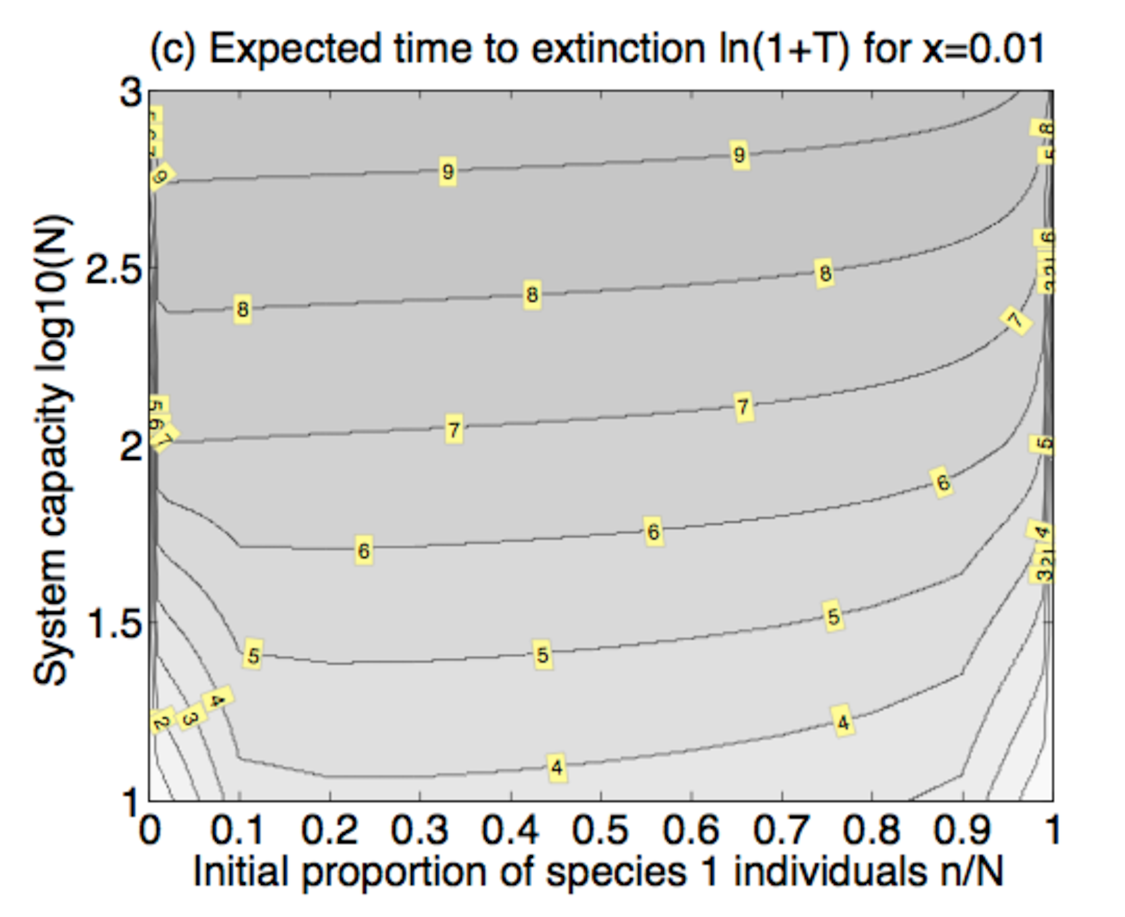
\includegraphics[width=2.5in]{x01resize.pdf} & 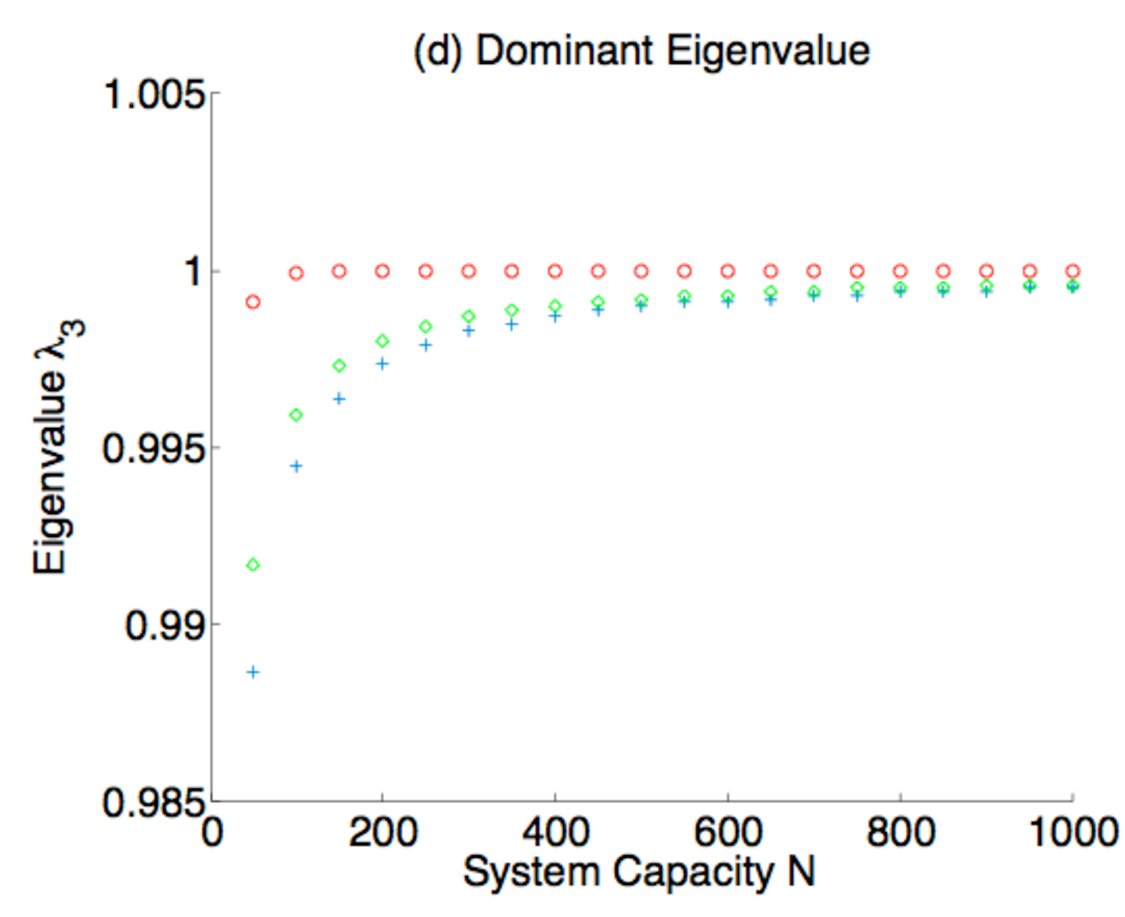
\includegraphics[width=2.5in]{domevalresize.pdf} \end{tabular}
   \caption[How time to extinction varies with system capacity]{(a-c) The expected time to extinction as it changes with system capacity $N$ for each initial population. In the region where invasion analysis suggests coexistence should occur, the increase in expected time to extinction with $N$ is greatest, although for all $x$, the increase is more rapid than the increase in system capacity. (d) The effect of system size on dominant eigenvalue $\lambda_3$ for $x>x_{max}$ (crosses), $x<x_{min}$ (diamonds) and $x \in(x_{min},x_{max})$ (circles). Growth rate when the system is away from the boundaries behaves like $\lambda_3^t$. As system capacity increases, $\lambda_3$ tends to 1, resulting in slower convergence to either the boundary or an interior quasi-equilibrium. Note that when $x \in (x_{min},x_{max}$, the convergence $\lambda_3 \to 1$ ccurs more rapidly than for $x$ outside this interval.}
 \label{fig:tte}
\end{figure}

We can also find the expected time to convergence (be that extinction or an internal quasi-equilibrium) by examining the eigenvalues of the transition matrix. The two absorbing boundaries mean that this matrix is reducible, with two eigenvalues $\lambda_{1,2}=1$, so the dynamics away from these boundaries are determined by $\lambda_3$, \textbf{the largest eigenvalue with $\lambda \neq 1$. The convergence to either the boundary or the quasi-equilibrium happens with rate $\lambda_3^t$. Figure\ref{fig:tte} shows numerically generated $\lambda_3$ for varied $x \in \{0.01,0.035,0.06\}$ above, below and within the non-disturbed coexistence region. In all cases, $\lambda^3$ increases monotonically with $N$. This indicates} that time to convergence increases with system size. When $x \not\in (x_{min},x_{max})$, this extends the time to extinction, allowing for less frequent disturbances to sustain both populations.



 \section{Differential seed productivity}
\label{app2c}
Suppose that not all individuals are reproductively active all the time. Instead, there is a probability  $p$ that an individual is producing seeds at that moment. This effectively reduces the amount of competition for a gap when one appears in the canopy.

We then consider the conditions for coexistence, i.e. \eqref{lowerboundarycond} and \eqref{upperboundarycond}.
We assume that when the system is almost entirely filled with one species, the seed production can be approximated by the mean, so in \eqref{lowerboundarycond} we assume the number of seeds produced by $N-2$ individuals of species 2 is given by $s_2 p (N-2)$. We can therefore solve \eqref{lowerboundarycond} for $x$. Note that a single individual of species 1 can produce either $s_1$ seeds (with probability $p$) or 0 seeds  (probability $1-p$). Using the relationship $P(A)=\sum_{b \in B}P(A|b)$, where $P(A)$ is the probability of species 1 increasing from one individual to two, and $B$ is the of all possible seed numbers produced by species 1 (here the set $\{ 0, s_1\}$), solving \eqref{lowerboundarycond} gives 
\begin{align*}
\ln \left( \frac{(N-1)ps_1}{s_1+ps_2(N-2)}\right) \frac{N}{ps_2(N-2)} &> x. \\
\end{align*}
Taking the limit as system capacity $N$ tends to infinity, we find that an upper bound for $x$ is given by
$$
x<\frac{\ln \left(\frac{s_1}{s_2}\right)}{p s_2}
$$
which merely differs by a factor of $1/p$ from the simpler base model.

Similarly, we can solve \eqref{upperboundarycond} for $x$ as follows:
\begin{align*}
 x&>\frac{N}{s_2}\ln \left( \frac{p^2 s_1(N-1)(N-2)}{((N-1)p-1)(ps_1(N-2)+s_2)} \right) \end{align*}

Again, taking the limit as system capacity $N\rightarrow \infty$ gives 
$$
x>\frac{s_1-s_2}{ps_1s_2}=\frac{1}{p}\left(\frac{1}{s_2}-\frac{1}{s_1}\right) $$
which again differs from the base model merely by a factor of $1/p$. Simulations confirm that between these boundaries, long term coexistence is observed.

\section{Comparison of simulation data with analytic predictions}
\label{app2d}
We ran a range of time series simulations to verify the predictions given by our analytical results. Simulations are run at $I=0.1,0.2,0.3,0.4,0.5,0.6,0.7,0.8,0.9$ and $1$ and frequencies $\ln(T_D)=1,2,3,4,5,6,7,8$. Each point has 20 simulations run for $10^5$ time steps, and a linear interpolation algorithm is used between data points. Dark colours in Figure~\ref{fig:simulationdata}(a) are indicative of high probability of coexistence, \textbf{where both species persist in the community after $10^5$ time steps.} The scale to the right shows the percentage of the 20 time series exhibit coexistence. This data indicates that while the outcomes are accurately predicted by the analysis when disturbance events are very frequent (Figure~\ref{fig:simulationdata}(b)), there is a ``tail'' at high intensity and intermediate frequency where coexistence is only possible for a very narrow range of frequencies. However, frequencies that are sufficiently high (such that the lines given by $\text{AverageChange}(1)=0$ and $\text{AverageChange}(N-1)=0$  are approximately constant in $\ln(T_D)$) the average change function provides a good fit to the simulation data (Figure~\ref{fig:simulationdata}). This is also the case for simulations in a system of size $N=10000$, where the average change provides a good fit for frequencies where the region of coexistence is approximately constant in $f$ (results not shown).
\begin{figure}\begin{tabular}{ll}
(a)&(b)\\
 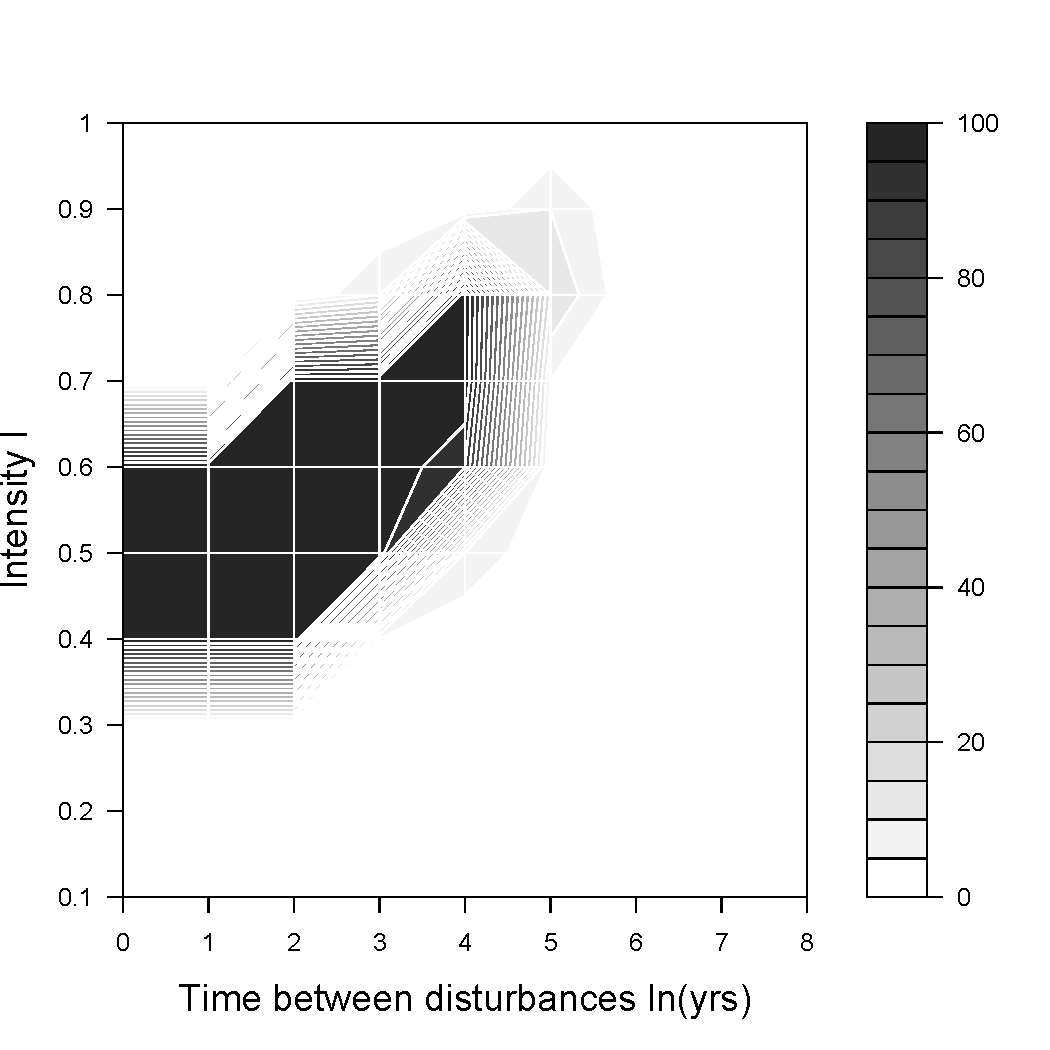
\includegraphics[width=2.5in]{simcoexist.pdf}& 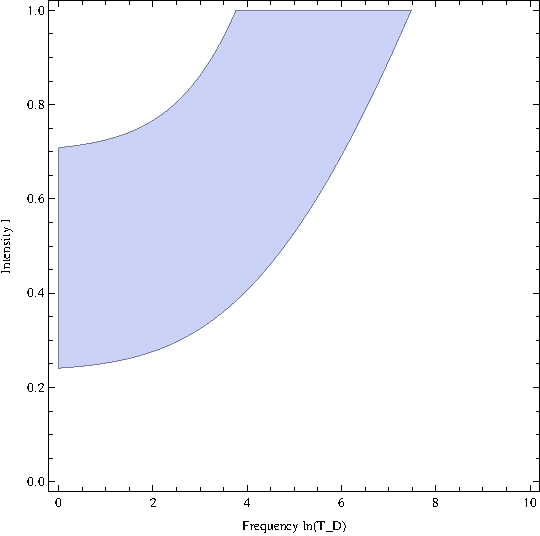
\includegraphics[width=2.5in]{hockeyTd.pdf}\end{tabular}
   \caption[Comparing simulation data with analytical predictions]{(a) Simulation data showing how stochasticity effects the predicted region of coexistence at high intensity. 20 time series simulations were run for each point. The darker the shading, the greater the number of these time series that exhibited coexistence after $10^5$ time steps. Linear scaling is performed between data points. (b) The region of coexistence predicted by invasion analysis. Parameters $s_1=500,s_2=50,x=0.06,N=1000$}
 \label{fig:simulationdata}
\end{figure}

\section{Approximation of expected change for $p<1$}
\label{app2e}
When not all individuals are reproductively active ($p<1$), the average change at the boundaries is given by
\begin{align}
\label{acd1}
&AvChangeDist(1)=-I \\ 
&+ (1-I)p \notag \\
& \times \sum_{k=0}^{N-2} k \sum_{j=k}^{N-2} I^j(1-I)^{N-2-j}{N-2\choose j} \sum_{r_2=0}^{N-1j}\\&\left( p^{r_2}(1-p)^{N-1-j-r_2} {N-1-j\choose r_2}\left( \frac{s_1 e^{-s_2xr_2/N}}{s_1+s_2r_2}\right)^k \left(1- \frac{s_1 e^{-s_2xr_2/N}}{s_1+s_2r_2}\right)^{j-k}{j\choose k} \right) \notag \\
&+(N-1)I^{N-1}(1-I) \notag
\end{align}
and
\begin{align}
\label{acdt}
&AvChangeDist(N-1)=-(N-1)I^{N-1}\\& - (1-I)p \notag \\
&\times \sum_{k=1}^{N-2}k\sum_{j=k}^{N-2} I^j(1-I)^{N-2-j} {N-2 \choose j} \sum_{r_1=0}^{N-1-j} \notag \\
&\left( p^{r_1}(1-p)^{N-1-j-r_1} {N-1-j\choose r_1}\left( \frac{s_1r_1 e^{-s_2x/N}}{s_2+s_1r_1}\right)^{j-k} \left(1- \frac{s_1r_1 e^{-s_2x/N}}{s_2+s_1r_1}\right)^k{j\choose k} \right) \notag \\
&+I(1-I^{N-1}) \notag
\end{align}
However, these are computationally expensive, where the number of terms in the triple sum scales as $N^3$, so as system size increases, the calculation of \eqref{acd1} and \eqref{acdt} rapidly becomes unfeasible. Instead, we use the normal approximation of the binomial distributions using the `integral2' function in Matlab2012b, to approximate the expected changes at the boundaries with 
\begin{align}
& AvChangeDistApprox(1)=-I \\
&+(1-I)p \notag \\
&\sum_{k=1}^{N-2} k \int_k^{N-2}dj \mathcal{N}\left(I(N-2),I(N-2)(1-I),j\right) \int_0^{N-1-j}dr_2 \mathcal{N}\left(p(N-1-j),p(1-p)(N-1-j),r_2\right) \notag \\
&\times \mathcal{N}\left(j\frac{s_1 e^{-s_2xr_2/N}}{s_1+s_2r_2},j\frac{s_1 e^{-s_2xr_2/N}}{s_1+s_2r_2}\left(1-\frac{s_1 e^{-s_2xr_2/N}}{s_1+s_2r_2}\right),k \right)\notag \\
 &+(N-1)I^{N-1}(1-I)\notag
\end{align}
at the lower boundary and 
\begin{align}
& AvChangeDistApprox(N-1)=-(N-1)I^{N-1}\\
& - (1-I)p \notag \\
& \sum_{k=1}^{N-2}k \int_k^{N-2}dj \mathcal{N}(I(N-2),I(1-I)(N-2),j)\int_0^{N-1-j}dr_1 \mathcal{N}(p(N-1-j),p(1-p)(N-1-j),r_1) \notag \\
& \times \mathcal{N}\left(j\left(1-\frac{s_1r_1 e^{-s_2x/N}}{s_2+s_1r_1}\right),j\frac{s_1r_1 e^{-s_2x/N}}{s_2+s_1r_1}\left(1-\frac{s_1r_1 e^{-s_2x/N}}{s_2+s_1r_1}\right)\right) \notag \\
&+I(1-I^{N-1})\notag \end{align}
at the upper boundary, where $\mathcal{N}(x,y,z)$ is the PDF of a normal distribution with mean $\mu=x$ and variance $\sigma^2=y$, analysed over the variable $z$.

The error for this approximation decreases with increased system capacity $N$. Evaluating for $I=0.1,0.2,...,0.9$ and $\ln(T_D)=1,2,...,8$, we find that the maximum error when $N=400$ is 0.0025, ensuring that even for relatively small $N>400$, this is a good approximation of the expected change.



\eappendix
